\section{Capítulo 3: Análisis}

En este capítulo se trabajará el análisis de los módulos de la aplicación para su correcto funcionamiento abarcando desde los límites y capacidades de la aplicación, así como los requerimientos, riesgos y mitigación de estos para tener una base sólida para el diseño y posterior desarrollo de nuestra solución.

\subsection{Alcance y Límites de la aplicación}

El propósito de este apartado es establecer de manera precisa el ámbito de desarrollo e implementación del proyecto. A continuación, se definen las capacidades operativas y el público objetivo que conforman el alcance del sistema, así como las restricciones técnicas, lingüísticas y de conectividad que delimitan su funcionamiento.

\subsubsection{Alcance de la aplicación web}

La aplicación web está dirigida exclusivamente a estudiantes de tercer y cuarto grado de educación primaria. La plataforma permitirá la recolección de textos manuscritos en letra de molde mediante la escritura directa en un lienzo en pantalla o a través de la carga de imágenes.

Una vez capturado, el texto será procesado mediante algoritmos de OCR para su digitalización, seguido por la intervención de un módulo de NLP encargado de analizar el contenido, detectar errores ortográficos y generar sugerencias automáticas de corrección.

Además, el sistema evaluará métricas cuantitativas del trazo manuscrito, considerando parámetros como la legibilidad, alineación, tamaño y espaciado.

\subsubsection{Límites de la aplicación web}

Las restricciones técnicas y operativas de la aplicación son en cuanto al estilo de escritura, el modelo de reconocimiento está estrictamente acotado al procesamiento de letra de molde (tipografía Century) \cite{ref40}, excluyendo la evaluación de letra cursiva u otras tipografías.

Respecto a la restricción lingüística, el análisis ortográfico y las sugerencias generadas se limitarán al nivel cognitivo y vocabulario correspondiente a los grados de tercero y cuarto de primaria.

En relación con el rol de la aplicación, el sistema funcionará exclusivamente como una herramienta de retroalimentación automatizada y complementaria, basada en un enfoque de aprendizaje ecléctico, sin sustituir la evaluación pedagógica integral del docente.

Finalmente, debido a su diseño basado en una arquitectura web cliente-servidor, existe una dependencia de conectividad, por lo que el funcionamiento de los módulos OCR y NLP requerirá una conexión activa a internet.


\subsection{Factibilidad}
 
El estudio de factibilidad es un instrumento que sirve para orientar la toma de decisiones en la evaluación de un proyecto. Se formula con base en información que tiene la menor incertidumbre posible para medir las posibilidades de éxito o fracaso, apoyándose en él se tomará la decisión de proceder o no con su implementación.
 
% ─────────────────────────────────────────────
\subsubsection{Factibilidad Técnica}
% ─────────────────────────────────────────────
 
La factibilidad técnica estudia la posibilidad tecnológica para que el proyecto pueda llevarse a cabo satisfactoriamente con el menor riesgo posible. Las herramientas tecnológicas se dividen en software y hardware.
 
\paragraph{Software}
 
El software es una parte esencial en la elaboración del proyecto, ya que con este se desarrollará la aplicación web y el servidor. Todas las herramientas seleccionadas tienen costo cero para el equipo, incluyendo GitHub en su plan gratuito, el cual cubre repositorios privados ilimitados, colaboradores ilimitados y 2{,}000 minutos mensuales de CI/CD, suficientes para un equipo de tres personas.
 
\begin{table}[H]
\centering
\caption{Herramientas de software para el desarrollo del proyecto.}
\label{tab:software}
\renewcommand{\arraystretch}{1.3}
\begin{tabularx}{\textwidth}{|l|X|l|r|r|}
\hline
\textbf{Herramienta} & \textbf{Uso en el proyecto} & \textbf{Tipo} & \textbf{Costo/mes} & \textbf{11 meses} \\
\hline
React / Next.js   & Front-End: panel tutor, panel alumno, lienzo digital  & Libre & \$0 & N/A \\
\hline
FastAPI (Python)  & Back-End: endpoints REST, lógica de negocio, JWT      & Libre & \$0 & N/A \\
\hline
SQL Server Express & Base de datos: tablas, triggers, vistas, restricciones & Libre & \$0 & N/A \\
\hline
Docker            & Contenedorización y despliegue                        & Libre & \$0 & N/A \\
\hline
VS Code           & Editor de código fuente                               & Libre & \$0 & N/A \\
\hline
GitHub (Free)     & Control de versiones, repos privados, CI/CD           & Libre & \$0 & N/A \\
\hline
GCP / AWS         & Hosting: prueba piloto en tier gratuito               & Libre & \$0 & N/A \\
\hline
\multicolumn{3}{|r|}{\textbf{Total}} & \multicolumn{2}{r|}{\textbf{\$0 MXN}} \\
\hline
\end{tabularx}
\end{table}
 
\paragraph{Hardware}
 
El hardware es fundamental para el desarrollo del proyecto. A continuación se presentan las especificaciones de los equipos de cómputo de cada integrante del equipo, los cuales serán utilizados durante todo el desarrollo.
 
\begin{table}[H]
\centering
\caption{Características de los equipos de cómputo y dispositivos de prueba.}
\label{tab:hardware}
\renewcommand{\arraystretch}{1.3}
\begin{tabularx}{\textwidth}{|X|X|c|c|c|r|}
\hline
\textbf{Equipo} & \textbf{Procesador} & \textbf{RAM} & \textbf{Almac.} & \textbf{SO} & \textbf{Valor ref. (MXN)} \\
\hline
Lenovo IdeaPad  & AMD Ryzen 7 & 16 GB & 512 GB SSD & Arch Linux & \$18,000 \\
\hline
MacBook Air     & Apple M1 & 8 GB & 256 GB SSD & macOS & \$28,000 \\
\hline
HP Spectre x360 & Intel Core i7 & 16 GB & 512 GB SSD & Windows 11 & \$25,000 \\
\hline
iPad / Tablets  & N/A & N/A & N/A & iPadOS/Android & \$10,000 \\
\hline
\multicolumn{5}{|r|}{\textbf{Total (valor de referencia — ya en posesión del equipo)}} & \textbf{\$81,000} \\
\hline
\end{tabularx}
\end{table}
 
Dadas las características de las herramientas tanto en software como en hardware, se puede observar que el proyecto puede llevarse a cabo correctamente. El stack tecnológico es coherente y moderno: React/Next.js cubre el front-end educativo, FastAPI con Python concentra la lógica de inteligencia artificial (OCR y NLP), y SQL Server garantiza integridad referencial con soporte a triggers y vistas. El Ryzen 7 y el M1 son los equipos más capaces para ejecutar los modelos localmente durante el desarrollo.
 
% ─────────────────────────────────────────────
\subsubsection{Factibilidad Operativa}
% ─────────────────────────────────────────────
 
La factibilidad operativa comprende una determinación de la probabilidad para que un proyecto se realice o funcione como se supone, considerando si se cuenta con el personal capacitado y los recursos humanos necesarios. Al realizar el análisis se calcula tanto el tiempo de esfuerzo como las horas dedicadas al sistema.
 
\begin{table}[H]
\centering
\caption{Resumen de días hábiles para el desarrollo del proyecto.}
\label{tab:dias}
\renewcommand{\arraystretch}{1.3}
\begin{tabularx}{\textwidth}{|l|r|r|r|r|r|r|}
\hline
\textbf{Mes} & \textbf{Días} & \textbf{Fin de semana} & \textbf{Días no laborales} & \textbf{Días hábiles} & \textbf{Hrs/día} & \textbf{Hrs totales} \\
\hline
Enero      & 31 & 9 & 1 & 21 & 4 & 84  \\
\hline
Febrero    & 28 & 8 & 1 & 19 & 4 & 76  \\
\hline
Marzo      & 31 & 8 & 1 & 22 & 4 & 88  \\
\hline
Abril      & 30 & 8 & 2 & 20 & 4 & 80  \\
\hline
Mayo       & 31 & 9 & 1 & 21 & 4 & 84  \\
\hline
Junio      & 30 & 8 & 0 & 22 & 4 & 88  \\
\hline
Julio      & 31 & 9 & 0 & 22 & 4 & 88  \\
\hline
Agosto     & 31 & 9 & 0 & 22 & 4 & 88  \\
\hline
Septiembre & 30 & 8 & 1 & 21 & 4 & 84  \\
\hline
\textbf{Total} & & & & \textbf{190} & & \textbf{760} \\
\hline
\end{tabularx}
\end{table}
 
Es necesaria la definición de roles en el desarrollo del proyecto para llevar una organización eficiente donde cada integrante desempeñe sus actividades sin generar retrasos. Dado que el equipo de trabajo cuenta con tres personas, es necesario que los integrantes desempeñen más de un rol a lo largo del proyecto.
 
\begin{table}[H]
\centering
\caption{Roles de trabajo del proyecto.}
\label{tab:roles}
\renewcommand{\arraystretch}{1.3}
\begin{tabularx}{\textwidth}{|l|X|r|}
\hline
\textbf{Rol} & \textbf{Descripción} & \textbf{Personas necesarias} \\
\hline
Líder de proyecto       & Encargado de la coordinación y planeación del proyecto.                                          & 1 \\
\hline
Analista / Arquitecto   & Realiza el análisis e diseño de la arquitectura del sistema y sus módulos.                       & 1 \\
\hline
Desarrollador Front-End & Desarrolla la interfaz de usuario con React/Next.js: paneles de tutor y alumno, lienzo digital.  & 1 \\
\hline
Desarrollador Back-End  & Implementa los endpoints REST con FastAPI, lógica de negocio, autenticación JWT y BCrypt.        & 1 \\
\hline
Especialista IA         & Integra y ajusta los módulos de OCR y NLP para análisis caligráfico y corrección ortográfica.    & 1 \\
\hline
Tester / QA             & Realiza las pruebas funcionales y de integración para validar el correcto funcionamiento.        & 1 \\
\hline
\end{tabularx}
\end{table}
 
A continuación se muestra la distribución del porcentaje de participación para cada rol y el promedio de días laborales correspondiente, tomando como base 190 días hábiles de desarrollo.
 
\begin{table}[H]
\centering
\caption{Porcentaje de participación de cada rol del proyecto.}
\label{tab:participacion}
\renewcommand{\arraystretch}{1.3}
\begin{tabularx}{\textwidth}{|X|r|r|}
\hline
\textbf{Rol} & \textbf{Porcentaje de participación} & \textbf{Días laborales} \\
\hline
Líder de proyecto       & 15\% & 28.5 días \\
\hline
Analista / Arquitecto   & 15\% & 28.5 días \\
\hline
Desarrollador Front-End & 20\% & 38.0 días \\
\hline
Desarrollador Back-End  & 20\% & 38.0 días \\
\hline
Especialista IA (OCR + NLP) & 20\% & 38.0 días \\
\hline
Tester / QA             & 10\% & 19.0 días \\
\hline
\end{tabularx}
\end{table}
 
La factibilidad operativa del proyecto se muestra positiva. Los días totales calculados son una estimación considerando una dedicación de 4 horas diarias promedio por integrante. Consideramos que el tiempo para el desarrollo tiene suficiente holgura siempre y cuando se sigan las actividades y los calendarios acordados, y se priorice la integración temprana entre módulos para detectar problemas antes de la prueba piloto con 25 alumnos.
 
% ─────────────────────────────────────────────
\subsubsection{Factibilidad Económica}
% ─────────────────────────────────────────────
 
Se toma en consideración el capital disponible para invertir en el desarrollo del proyecto. Se determina el presupuesto de costos de los recursos técnicos, humanos y materiales tanto para el desarrollo como para la implantación. El sueldo de referencia utilizado es de \$20{,}000 MXN mensuales por desarrollador de nivel junior a intermedio en México para el año 2025 \cite{occmundial2025salarios}.
 
En primer lugar, se presentan los costos de las herramientas de software, los cuales son en su totalidad de costo cero para el equipo de desarrollo.
 
\begin{table}[H]
\centering
\caption{Estimación de costos de herramientas de software.}
\label{tab:costos-software}
\renewcommand{\arraystretch}{1.3}
\begin{tabularx}{\textwidth}{|X|r|r|}
\hline
\textbf{Herramienta} & \textbf{Costo mensual (MXN)} & \textbf{Costo por 9 meses (MXN)} \\
\hline
React / Next.js, FastAPI, SQL Server Express, Docker, VS Code, Figma, Postman, GitHub Free, GCP/AWS (tier gratuito) & \$0 & \$0 \\
\hline
\textbf{Total} & \textbf{\$0} & \textbf{\$0} \\
\hline
\end{tabularx}
\end{table}
 
A continuación se presentan los costos de los servicios necesarios para llevar a cabo el proyecto.
 
\begin{table}[H]
\centering
\caption{Costos de servicios.}
\label{tab:servicios}
\renewcommand{\arraystretch}{1.3}
\begin{tabularx}{\textwidth}{|X|r|r|}
\hline
\textbf{Servicio} & \textbf{Costo por mes (MXN)} & \textbf{Costo por 9 meses (MXN)} \\
\hline
Electricidad e internet (3 integrantes × \$800) & \$2{,}400 & \$21{,}600 \\
\hline
Infraestructura en nube (GCP / AWS — tier gratuito en piloto) & \$0 & \$0 \\
\hline
\textbf{Total} & \textbf{\$2{,}400} & \textbf{\$21{,}600} \\
\hline
\end{tabularx}
\end{table}
 
Finalmente, en la Tabla \ref{tab:costos-total} se presenta el resumen de costos totales del proyecto.
 
\begin{table}[H]
\centering
\caption{Resumen de costos totales del proyecto.}
\label{tab:costos-total}
\renewcommand{\arraystretch}{1.3}
\begin{tabularx}{\textwidth}{|X|r|}
\hline
\textbf{Concepto} & \textbf{Costo total (MXN)} \\
\hline
Sueldos — costo comercial equivalente (3 personas × 9 meses × \$20{,}000) & \$540{,}000 \\
\hline
Equipo de cómputo (valor de referencia — ya en posesión del equipo)        & \$61{,}000 \\
\hline
Servicios (electricidad e internet, 9 meses)                               & \$21{,}600 \\
\hline
Herramientas de software                                                   & \$0        \\
\hline
Infraestructura en nube                                                    & \$0        \\
\hline
\textbf{Total}                                                             & \textbf{\$622{,}600} \\
\hline
\end{tabularx}
\end{table}
 
Con base en la tabla anterior, se puede concluir que el costo comercial equivalente del proyecto asciende a \$622{,}600 MXN. Sin embargo, al ser este un trabajo terminal, los sueldos (que representan el 86.7\% del total) son absorbidos por el propio equipo como parte de su formación académica, y el hardware ya se encuentra en posesión de los integrantes. El desembolso directo real del equipo se limita a los servicios básicos de electricidad e internet, estimados en \$21{,}600 MXN durante los 9 meses de desarrollo, siendo el resto de las herramientas completamente gratuitas.
\subsubsection{Factibilidad Legal}

La implementación del sistema requiere observar un conjunto de disposiciones jurídicas del ordenamiento mexicano que regulan directamente tres ámbitos: la protección de datos personales de menores de edad, los derechos de niñas, niños y adolescentes en entornos tecnológicos, y la propiedad intelectual del software académico. A continuación se analiza cada uno de estos marcos normativos y su aplicación concreta al sistema propuesto.

\subsubsection*{A. Protección de datos personales de menores de edad}
El tratamiento de los datos generados por el sistema — incluyendo muestras de escritura manuscrita, credenciales de acceso, resultados de análisis y métricas de desempeño — constituye tratamiento de datos personales en los términos de la Ley Federal de Protección de Datos Personales en Posesión de los Particulares (LFPDPPP), publicada originalmente en el Diario Oficial de la Federación el 5 de julio de 2010 y actualizada mediante la versión publicada el 20 de marzo de 2025, vigente a partir del 21 de marzo de 2025 \cite{lfpdppp2025}.

Dado que los usuarios finales son estudiantes de tercer y cuarto grado de educación primaria (entre 8 y 10 años de edad), se trata de datos personales de menores de edad, categoría que la ley somete a un régimen reforzado de protección. Los artículos específicos del ordenamiento que aplican al presente sistema son los siguientes:

\textbf{Artículo 7 (Consentimiento para menores de edad).} \\
La LFPDPPP establece que en el tratamiento de datos personales de menores de edad se deberá privilegiar el interés superior de la niña, el niño y el adolescente \cite{lfpdppp2025}. En concordancia con ello, la reforma de 2025 obliga expresamente a que el consentimiento para tratar datos de menores sea otorgado por padres, madres o tutores legales \cite{lfpdppp2025}. El sistema atiende este requerimiento mediante la figura del Tutor como actor principal del registro: únicamente el tutor autenticado puede dar de alta alumnos en la plataforma (RN-02), vinculando cada alumno a un responsable legal que actúa como representante en el tratamiento de sus datos (RN-03). Esto satisface el requisito de consentimiento informado, específico y libre exigido por la ley.

\textbf{Artículo 19 y 20 (Medidas de seguridad técnica, administrativa y física).} \\
La LFPDPPP obliga al responsable del tratamiento a implementar medidas de seguridad administrativas, técnicas y físicas que protejan los datos personales contra daño, pérdida, alteración, destrucción o acceso no autorizado \cite{lfpdppp2025}. El sistema da cumplimiento a este requerimiento mediante tres mecanismos: (1) autenticación basada en tokens JWT que impiden el acceso no autorizado a los datos de cada usuario según su rol; (2) almacenamiento de contraseñas mediante algoritmos de hash BCrypt (campo \texttt{contrasena\_cifrada} de tipo VARCHAR(255) en la tabla Usuarios); y (3) una arquitectura de separación de roles que garantiza que un alumno solo puede visualizar sus propios resultados (RN-25) y que únicamente el tutor responsable puede consultar y modificar los resultados de sus alumnos (RN-24).

\textbf{Derechos ARCO (Artículos 28--37).} \\
La ley reconoce a los titulares los derechos de Acceso, Rectificación, Cancelación y Oposición (ARCO) respecto de sus datos personales \cite{lfpdppp2025}. Para el ejercicio de estos derechos por parte de menores de edad, la ley dispone que deberá realizarse a través de su representante legal \cite{lfpdppp2025}. En el sistema, el tutor puede modificar los resultados de ejercicios de sus alumnos (RU-18) y el diseño contempla bajas lógicas en lugar de eliminación física de registros (RN-09), lo que permite la cancelación de datos sin comprometer la integridad referencial del sistema.

\textbf{Aviso de privacidad.} \\
El sistema deberá incorporar un aviso de privacidad accesible dentro de la interfaz, con lenguaje claro y adaptado al nivel educativo de los usuarios, informando sobre el responsable del tratamiento, las finalidades del uso de los datos, los mecanismos para el ejercicio de los derechos ARCO y el periodo de conservación de la información, en cumplimiento de los principios de licitud, información y proporcionalidad establecidos en la LFPDPPP \cite{lfpdppp2025}.

\subsubsection*{B. Derechos de niñas, niños y adolescentes en entornos tecnológicos}
La Ley General de los Derechos de Niñas, Niños y Adolescentes (LGDNNA), publicada en el Diario Oficial de la Federación el 4 de diciembre de 2014 y reformada por última vez el 27 de mayo de 2024, establece un catálogo de 20 derechos fundamentales aplicables a todas las personas menores de 18 años en territorio mexicano \cite{lgdnna2024}.

Dos artículos de esta ley resultan directamente relevantes para el presente proyecto:

\textbf{Artículo 13, fracción XX (Derecho de acceso a las Tecnologías de la Información y Comunicación).} \\
La LGDNNA reconoce expresamente el derecho de niñas, niños y adolescentes al acceso a las tecnologías de la información y comunicación, así como a los servicios de radiodifusión y telecomunicaciones, incluido el de banda ancha e internet, sin discriminación de ningún tipo o condición \cite{lgdnna2024}. El presente sistema se alinea con este derecho al constituir una herramienta educativa digital orientada a fortalecer competencias de escritura, ampliando las posibilidades de acceso a recursos tecnológicos dentro del entorno escolar de educación básica.

\textbf{Artículo 18 (Interés superior de la niñez como principio rector).} \\
La ley establece que en todas las medidas concernientes a niñas, niños y adolescentes se tomará en cuenta como consideración primordial su interés superior \cite{lgdnna2024}. Este principio se materializa en el diseño pedagógico del sistema: los ejercicios están basados en los programas de estudio de la SEP para tercer y cuarto grado, la retroalimentación automatizada es constructiva y no punitiva, y la interfaz está diseñada para minimizar la carga cognitiva y la frustración del estudiante.

\subsubsection*{C. Propiedad intelectual y licencias de software}
El desarrollo del sistema se enmarca en el régimen de Trabajo Terminal de la Escuela Superior de Cómputo (ESCOM) del Instituto Politécnico Nacional, cuyas normativas institucionales establecen que los derechos patrimoniales de los productos académicos generados corresponden a la institución, mientras que los autores conservan sus derechos morales \cite{escom_tt}.

Respecto al uso de herramientas de terceros, todas las tecnologías seleccionadas para el desarrollo cuentan con licencias compatibles con fines académicos y no comerciales:

\begin{itemize}
    \item \textbf{Tesseract OCR:} Licencia Apache 2.0, que permite uso, modificación y distribución sin restricciones para fines académicos.
    \item \textbf{FastAPI:} Licencia MIT, de uso libre sin condiciones.
    \item \textbf{React:} Licencia MIT.
    \item \textbf{Dataset Letras Alfabeto Español (Kaggle – Herrera, 2023):} Publicado bajo licencia Creative Commons, compatible con uso académico.
    \item \textbf{EMNIST:} Publicado por el NIST como dataset de acceso público para investigación.
\end{itemize}

El uso de estos componentes bajo sus respectivas licencias no genera obligaciones comerciales ni conflictos de propiedad intelectual con el marco institucional del proyecto.

\subsubsection*{D. Normatividad educativa}
El contenido pedagógico de los ejercicios y el análisis ortográfico del sistema se fundamentan en los programas de estudio de la Secretaría de Educación Pública (SEP) para educación básica — específicamente en los libros \textit{Nuestros Saberes} de tercer y cuarto grado (ciclo escolar 2025–2026) — lo que valida legalmente su pertinencia curricular dentro del sistema educativo nacional.

\subsubsection*{E. Síntesis de cumplimiento normativo}
En la Tabla \ref{tab:cumplimiento_normativo} se presenta un resumen del cumplimiento normativo del sistema respecto a las disposiciones legales identificadas como aplicables.

\begin{table}[H]
\centering
\caption{Síntesis de cumplimiento normativo del sistema.}
\label{tab:cumplimiento_normativo}
\renewcommand{\arraystretch}{1.5}
\begin{tabular}{|>{\centering\arraybackslash}m{3.5cm}|>{\centering\arraybackslash}m{4.5cm}|>{\centering\arraybackslash}m{7cm}|}
\hline
\textbf{Marco normativo} & \textbf{Artículo(s) aplicable(s)} & \textbf{Mecanismo de cumplimiento en el sistema} \\ \hline
LFPDPPP (2025) & Art. 7 --- Consentimiento de menores & Registro de alumnos exclusivamente por el tutor responsable (RN-02, RN-03) \\ \hline
LFPDPPP (2025) & Arts. 19--20 --- Seguridad técnica & JWT, BCrypt, separación de roles (RN-24, RN-25) \\ \hline
LFPDPPP (2025) & Arts. 28--37 --- Derechos ARCO & Modificación de resultados por tutor (RU-18), baja lógica (RN-09) \\ \hline
LGDNNA (2024) & Art. 13 fracc. XX --- Acceso a TIC & Herramienta digital educativa de acceso supervisado \\ \hline
LGDNNA (2024) & Art. 18 --- Interés superior & Diseño pedagógico basado en programas SEP, retroalimentación constructiva \\ \hline
Reglamento ESCOM-IPN & Propiedad intelectual académica & Derechos patrimoniales al IPN, derechos morales a los autores \\ \hline
Licencias de software de terceros & Apache 2.0, MIT, CC & Uso académico sin restricciones en todos los componentes \\ \hline
Programas SEP 3.$^{\circ}$ y 4.$^{\circ}$ grado & Plan de Estudios 2017 / Nuestros Saberes 2024 & Ejercicios diseñados con base en contenidos curriculares oficiales \\ \hline
\end{tabular}
\end{table}

En razón de lo anterior, el proyecto se considera legalmente factible. El diseño del sistema contempla de forma explícita los requerimientos normativos vigentes en materia de protección de datos de menores, derechos digitales de la infancia y propiedad intelectual académica, sin que ninguna disposición identificada represente un impedimento para su desarrollo o despliegue en un entorno educativo supervisado.

\clearpage % Para asegurar que la tabla no se desborde a la siguiente sección
\subsection{Requerimientos del usuario.}

En esta sección se describen los requerimientos del usuario, los cuales representan las expectativas y servicios que esperan los usuarios finales de la aplicación web. Estos requerimientos han sido identificados con base al análisis del problema, con el objetivo de propiciar que la solución desarrollada sea útil.

Los requerimientos del usuario se definen, de manera general, qué debe hacer la aplicación web desde la perspectiva del usuario en un lenguaje natural, sin entregar detalles técnicos de implementación. Estos servirán como base para la definición de requerimientos funcionales y no funcionales. 

\begin{tabularx}{\textwidth}{|>{\centering\arraybackslash}m{2cm}|m{3.6cm}|Y|>{\centering\arraybackslash}m{2.0cm}|}
\caption{Requerimientos del usuario.}
\label{tab:ru} \\

\hline
\textbf{ID} & \textbf{Nombre} & \textbf{Descripción} & \textbf{Prioridad} \\
\hline
\endfirsthead

\hline
\textbf{ID} & \textbf{Nombre} & \textbf{Descripción} & \textbf{Prioridad} \\
\hline
\endhead

\hline
\endfoot

% RU-01
RU-01 &
Registro de usuarios. &
La aplicación web debe permitir el registro de usuarios. El tutor se registra de forma autónoma, mientras que los alumnos son registrados por el tutor, asociándolos a su grado y grupo. &
Alta \\
\hline

% RU-02
RU-02 &
Autenticación de usuario. &
El usuario debe poder autenticarse en la aplicación web para acceder a sus funcionalidades de acuerdo con su rol. &
Alta \\
\hline

% RU-03
RU-03 &
Visualización de estado de alumnos. &
El tutor debe poder visualizar el estado de desempeño de sus alumnos, clasificándolos como bajo desempeño, desempeño regular y desempeño de excelencia, con el fin de identificar su progreso. &
Alta \\
\hline

% RU-04
RU-04 &
Clasificación de alumnos. &
La aplicación web debe mostrar un gráfico con la cantidad de alumnos clasificados según su nivel de desempeño (bajo, regular y excelencia), actualizándose conforme a los resultados obtenidos en ortografía y legibilidad. &
Media \\
\hline

% RU-05
RU-05 &
Visualización de ejercicios. &
La aplicación web debe permitir observar los ejercicios disponibles. &
Alta \\
\hline

% RU-06
RU-06 &
Activación de ejercicios. &
El tutor debe poder activar ejercicios a su elección, estableciendo una fecha límite de entrega cuando lo considere necesario. &
Alta \\
\hline

% RU-07
RU-07 &
Visualización de ejercicios seleccionados. &
La aplicación web debe mostrar los ejercicios seleccionados por el tutor y su fecha límite de entrega. &
Media \\
\hline

% RU-08
RU-08 &
Visualización de ejercicios pendientes. &
El alumno debe poder observar los ejercicios asignados y su fecha límite de entrega, para una correcta organización y cumplimiento de sus actividades en tiempo. &
Alta \\
\hline

% RU-09
RU-09 &
Visualización de ejercicios vencidos por tutor. &
La aplicación web debe permitir al tutor consultar los ejercicios cuya fecha límite ha expirado, para poder extender el plazo de entrega si lo considera necesario. &
Media \\
\hline

% RU-10
RU-10 &
Visualización de ejercicios vencidos por alumno. &
El alumno debe poder observar los ejercicios que no completó a tiempo, para conocer su estado y saber si el tutor ya habilitó su entrega. &
Media \\
\hline

% RU-11
RU-11 &
Realizar intento de ejercicios pendientes. &
El alumno debe poder realizar el ejercicio seleccionado por el tutor en una vista de captura de escritura. &
Alta \\
\hline

% RU-12
RU-12 &
Escritura digital en lienzo. &
El alumno debe poder escribir directamente sobre un lienzo digital, contando con herramientas de goma y deshacer para corregir su trazo, con el fin de realizar el ejercicio de escritura manuscrita desde el dispositivo. &
Alta \\
\hline

% RU-13
RU-13 &
Carga de fotografía como alternativa. &
El alumno debe poder subir una fotografía de su escritura manuscrita en papel como alternativa al lienzo digital, para adaptarse a distintas condiciones de acceso. &
Alta \\
\hline

% RU-14
RU-14 &
Envío del ejercicio para revisión. &
El alumno debe poder enviar su ejercicio a la aplicación web para que sea analizado, una vez que considere que su escritura está lista. &
Alta \\
\hline

% RU-15
RU-15 &
Visualización de ejercicios completados. &
El alumno debe poder observar los ejercicios completados, así como sus resultados de escritura. &
Media \\
\hline

% RU-16
RU-16 &
Visualización de ejercicios completados por alumno. &
La aplicación web debe permitir al tutor observar las actividades realizadas por cada alumno, incluyendo sus resultados. &
Media \\
\hline

% RU-17
RU-17 &
Modificación de resultados. &
El tutor debe poder modificar los resultados de un ejercicio realizado por el alumno, en caso de no estar de acuerdo con el análisis ortográfico y caligráfico. &
Baja \\
\hline

% RU-18
RU-18 &
Visualización de actividades sugeridas. &
El alumno debe poder observar las actividades sugeridas por la aplicación web, correspondientes a sus análisis ortográficos y caligráficos. &
Media \\
\hline

% RU-19
RU-19 &
Realizar actividades sugeridas. &
El alumno debe poder realizar las actividades sugeridas por la aplicación web, para trabajar en la mejora de los aspectos detectados en su escritura. &
Media \\
\hline

\end{tabularx}

%------- Reglas de negocio

\subsection{Reglas de negocio}

\begin{tabularx}{\textwidth}{|>{\centering\arraybackslash}m{2cm}|m{3.6cm}|Y|>{\centering\arraybackslash}m{2.0cm}|}
\caption{Reglas de negocio.}
\label{tab:rn} \\

\hline
\textbf{ID} & \textbf{Nombre} & \textbf{Descripción}  \\
\hline
\endfirsthead

\hline
\textbf{ID} & \textbf{Nombre} & \textbf{Descripción}  \\
\hline
\endhead

\hline
\endfoot

RN-01 & Registro de tutores &
Todo usuario que actúe como tutor debe estar registrado en el sistema con el rol de tutor. \\ \hline

RN-02 & Registro de alumnos &
Todo alumno debe estar registrado en el sistema para poder realizar intentos y consultar resultados. \\ \hline

RN-03 & Tutor único por alumno &
Cada alumno debe tener exactamente un tutor asignado. \\ \hline

RN-04 & Tutor con múltiples alumnos &
Un tutor puede estar asociado a uno o más alumnos. \\ \hline

RN-05 & Correo obligatorio para tutores &
Todo tutor debe proporcionar un correo electrónico válido. \\ \hline

RN-06 & Integridad tutor--alumno &
No se permite registrar un alumno sin asignarlo a un tutor existente. \\ \hline

RN-07 & Persistencia de datos &
La información de alumnos, tutores, intentos y resultados debe conservarse de manera persistente. \\ \hline

RN-08 & Baja lógica de usuarios &
La eliminación de usuarios debe realizarse de forma lógica (cambio de estado) y no física. \\ \hline

RN-09 & Asociación de intento &
Cada intento debe estar asociado a un único alumno y a un único ejercicio. \\ \hline

RN-10 & Evidencia obligatoria del intento &
Cada intento debe incluir una evidencia asociada. \\ \hline

RN-11 & Registro de fecha y hora &
Cada intento debe almacenar la fecha y hora en que fue enviado. \\ \hline

RN-12 & Análisis caligráfico único &
Cada intento debe generar exactamente un análisis caligráfico. \\ \hline

RN-13 & Análisis ortográfico único &
Cada intento debe generar exactamente un análisis ortográfico. \\ \hline

RN-14 & Generación automática de análisis &
Los análisis del intento deben generarse automáticamente a partir del contenido del intento. \\ \hline

RN-15 & Métricas caligráficas mínimas &
El análisis caligráfico debe evaluar, como mínimo: alineación, tamaño, inclinación y espaciado. \\ \hline

RN-16 & Rango de métricas caligráficas &
Cada métrica caligráfica debe tener un valor dentro del rango de 0 a 10. \\ \hline

RN-17 & Observaciones del análisis &
El análisis caligráfico puede incluir observaciones adicionales generadas por el tutor. \\ \hline

RN-18 & Detección de errores ortográficos &
El análisis ortográfico debe detectar errores ortográficos en el texto del intento. \\ \hline

RN-19 & Conteo de errores &
El sistema debe almacenar el conteo total de errores ortográficos detectados por intento. \\ \hline

RN-20 & Sugerencias de corrección &
El sistema debe generar sugerencias de corrección ortográfica. \\ \hline

RN-21 & Puntuación ortográfica &
El análisis ortográfico debe asignar una puntuación ortográfica basada en los errores detectados dentro del rango de 0 a 10. \\ \hline

RN-22 & Historial y progreso del alumno &
El historial y el progreso del alumno deben generarse a partir de los datos de análisis de sus intentos. \\ \hline

RN-23 & Consulta por tutor &
Un tutor puede consultar los resultados de los alumnos a su cargo. \\ \hline

RN-24 & Modificación por tutor &
Un tutor puede modificar los resultados de los alumnos a su cargo únicamente si la política del sistema lo permite y queda registro del cambio. \\ \hline

RN-25 & Consulta por alumno &
Un alumno solo puede visualizar sus propios resultados. \\ \hline

RN-26 & Condición para ejercicio correctivo &
Un ejercicio correctivo automático solo puede generarse si el conteo de errores del intento es menor que 5. \\ \hline

RN-27 & Disponibilidad de impresión &
Todo ejercicio debe poder renderizarse para visualización e impresión/exportación. \\ \hline

\end{tabularx}

%---------- Casos de uso

\subsection{Modelado de casos de uso}
El modelado de casos de uso se utiliza ampliamente para apoyar la adquisición de requerimientos. Un caso de uso puede tomarse como un simple escenario que describa lo que espera el usuario de un sistema.

Cada caso de uso representa una tarea discreta que implica interacción externa con un sistema. En su forma más simple, un caso de uso se muestra como una elipse, con los actores que intervienen en el caso de uso representados como figuras humanas \cite{sommerville2015software}. 

\subsubsection{Diagrama de casos de uso }

\begin{figure}[H]
  \centering
  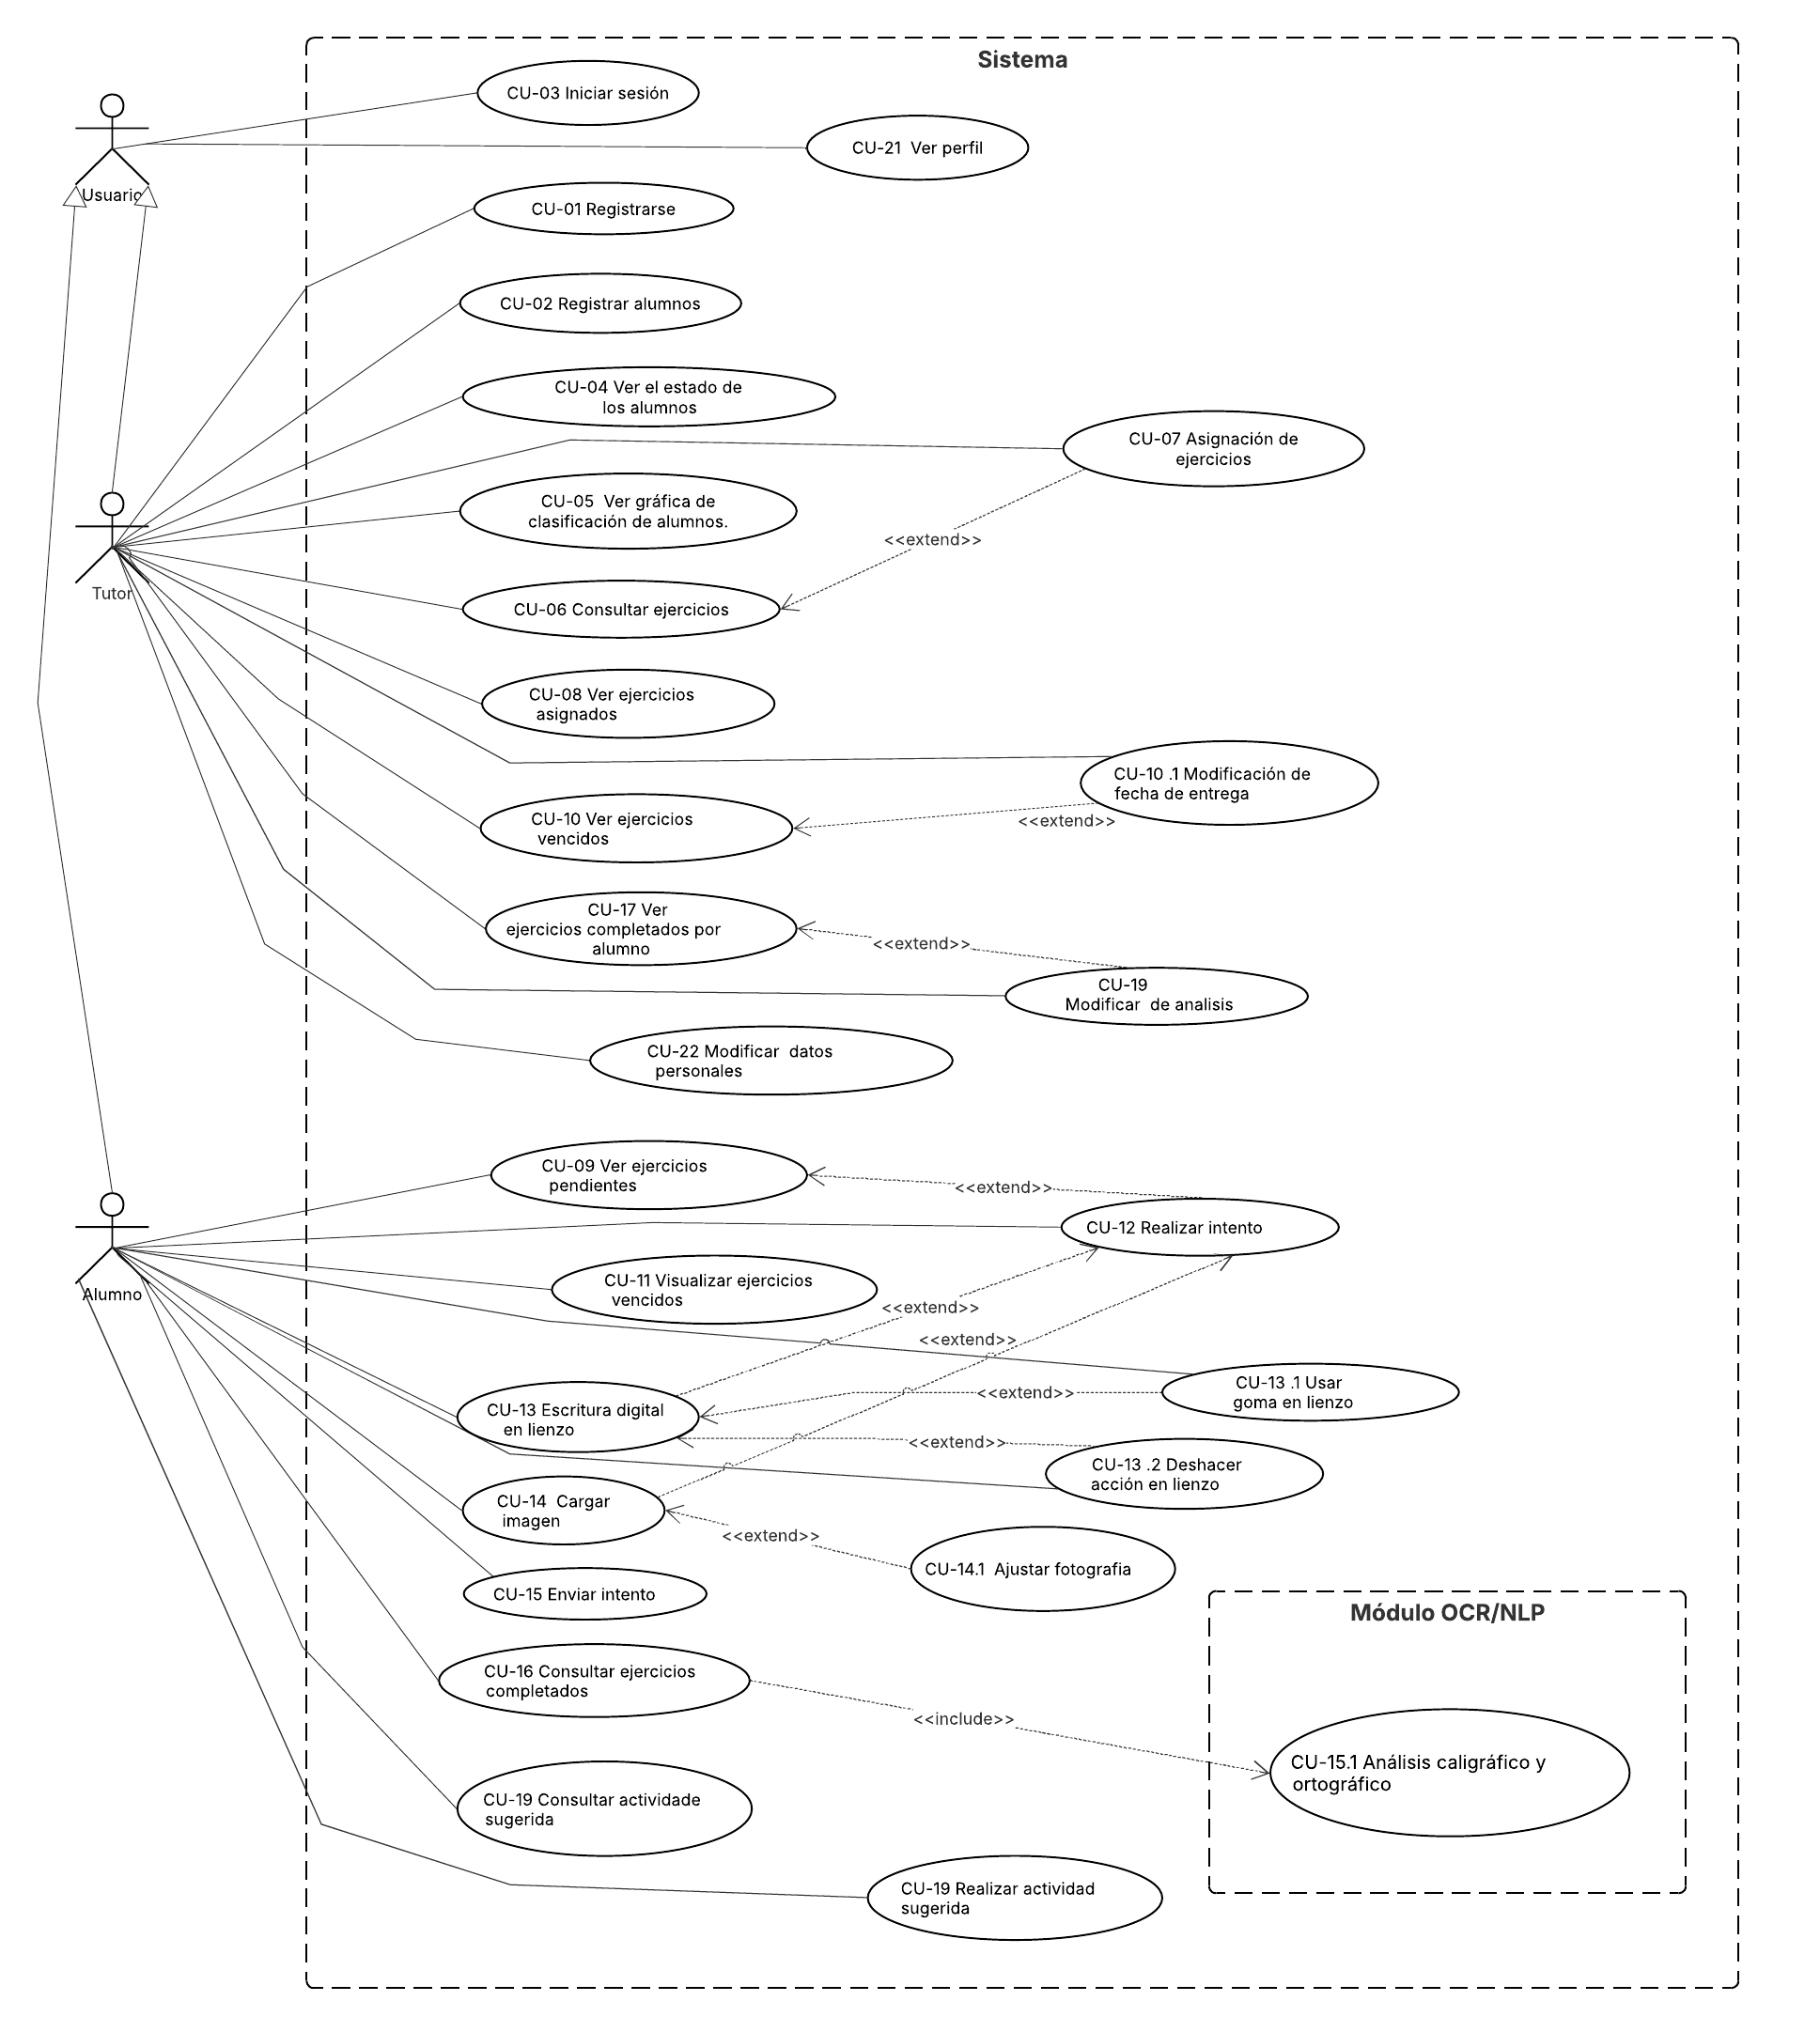
\includegraphics[height=0.82\textheight,keepaspectratio]{Imagenes/DiagramaCU-3.png}
  \caption{Diagrama de casos de uso}
\end{figure}

\subsubsection{Especificación de los casos de uso}

\begin{longtable}{|p{4cm}|p{11cm}|}
\caption{Tabla de especificación CU-01}
\label{tab:cu01} \\

\hline
\multicolumn{2}{|c|}{\textbf{CU-01 Registro de tutor}} \\
\hline
\endfirsthead

\hline
\multicolumn{2}{|c|}{\textbf{CU-01 Registro de tutor}} \\
\hline
\endhead

\hline
\endfoot

Actor & Tutor \\
\hline

Descripción & El tutor ingresa sus datos personales en el formulario de la aplicación web para crear su cuenta y acceder a sus funcionalidades. \\
\hline

Datos & Nombre, apellido paterno, nombre de usuario, correo electrónico, contraseña. \\
\hline

Estímulo & El tutor ingresa a la vista de registro, ingresa sus datos en el formulario y los envía. \\
\hline

Respuesta & La aplicación web valida los datos, crea la cuenta del tutor y le permite acceder a las funcionalidades del tutor. \\
\hline

Comentarios & El correo electrónico y nombre de usuario debe ser único en la aplicación web. \\
\hline

\end{longtable}

\begin{longtable}{|p{4cm}|p{11cm}|}
\caption{Tabla de especificación CU-02}
\label{tab:cu02} \\

\hline
\multicolumn{2}{|c|}{\textbf{CU-02 Registrar alumno}} \\
\hline
\endfirsthead

\hline
\multicolumn{2}{|c|}{\textbf{CU-02 Registrar alumno}} \\
\hline
\endhead

\hline
\endfoot

Actor & Tutor \\
\hline
Descripción & El tutor registra a un alumno en la aplicación web, ingresando sus datos e indicando el grado y grupo al que pertenece. \\
\hline
Datos & Nombre, apellido paterno, apellido materno, nombre de usuario, contraseña, grado y grupo. \\
\hline
Estímulo & El tutor, ya autenticado, ingresa a la vista ``Alumnos'', captura los datos en el formulario ``Alta de alumno'' y los envía. \\
\hline
Respuesta & La aplicación web registra los datos del alumno y lo asocia con el tutor responsable. \\
\hline
Comentarios & El nombre de usuario del alumno debe ser único. Solo tutores registrados pueden dar de alta alumnos. \\
\hline

\end{longtable}

%------------------------------------------------------

\begin{longtable}{|p{4cm}|p{11cm}|}
\caption{Tabla de especificación CU-03}
\label{tab:cu03} \\

\hline
\multicolumn{2}{|c|}{\textbf{CU-03 Iniciar sesión}} \\
\hline
\endfirsthead

\hline
\multicolumn{2}{|c|}{\textbf{CU-03 Iniciar sesión}} \\
\hline
\endhead

\hline
\endfoot

Actor & Tutor, Alumno \\
\hline
Descripción & El usuario ingresa sus credenciales para autenticarse y acceder a las funcionalidades según su rol. \\
\hline
Datos & Nombre de usuario y contraseña. \\
\hline
Estímulo & El usuario accede a la aplicación e ingresa sus credenciales en el formulario de inicio de sesión. \\
\hline
Respuesta & La aplicación valida las credenciales, identifica el rol y redirige a la vista correspondiente. \\
\hline
Comentarios & Si las credenciales son incorrectas, se muestra un mensaje de error. \\
\hline

\end{longtable}

%------------------------------------------------------

\begin{longtable}{|p{4cm}|p{11cm}|}
\caption{Tabla de especificación CU-04}
\label{tab:cu04} \\

\hline
\multicolumn{2}{|c|}{\textbf{CU-04 Ver el estado de los alumnos}} \\
\hline
\endfirsthead

\hline
\multicolumn{2}{|c|}{\textbf{CU-04 Ver el estado de los alumnos}} \\
\hline
\endhead

\hline
\endfoot

Actor & Tutor \\
\hline
Descripción & El tutor consulta el estado de desempeño de sus alumnos clasificados como bajo, regular y excelencia. \\
\hline
Datos & Lista de alumnos clasificados y métricas de progreso. \\
\hline
Estímulo & El tutor autenticado accede a su panel principal. \\
\hline
Respuesta & La aplicación muestra la lista de alumnos agrupados por categoría de desempeño. \\
\hline
Comentarios & Solo se muestran alumnos asociados al tutor autenticado. \\
\hline

\end{longtable}

%------------------------------------------------------

\begin{longtable}{|p{4cm}|p{11cm}|}
\caption{Tabla de especificación CU-05}
\label{tab:cu05} \\

\hline
\multicolumn{2}{|c|}{\textbf{CU-05 Ver gráfica de clasificación de alumnos}} \\
\hline
\endfirsthead

\hline
\multicolumn{2}{|c|}{\textbf{CU-05 er gráfica de clasificación de alumnos}} \\
\hline
\endhead

\hline
\endfoot

Actor & Tutor \\
\hline
Descripción & La aplicación presenta al tutor un gráfico con la distribución de alumnos según su nivel de desempeño. \\
\hline
Datos & Cantidad de alumnos en bajo, regular y excelencia. \\
\hline
Estímulo & El tutor accede al panel principal donde se muestra el gráfico. \\
\hline
Respuesta & La aplicación genera y actualiza dinámicamente el gráfico. \\
\hline
Comentarios & Puede mostrarse mediante gráfica de barras o anillo. \\
\hline

\end{longtable}

%------------------------------------------------------

\begin{longtable}{|p{4cm}|p{11cm}|}
\caption{Tabla de especificación CU-06}
\label{tab:cu06} \\

\hline
\multicolumn{2}{|c|}{\textbf{CU-06 Consultar ejercicios}} \\
\hline
\endfirsthead

\hline
\multicolumn{2}{|c|}{\textbf{CU-06 Consultar ejercicios}} \\
\hline
\endhead

\hline
\endfoot

Actor & Tutor \\
\hline
Descripción & La aplicación presenta al tutor el catálogo de ejercicios disponibles para asignar. \\
\hline
Datos & Nombre, descripción y contenido base del ejercicio. \\
\hline
Estímulo & El tutor accede a la sección de ejercicios. \\
\hline
Respuesta & La aplicación despliega el catálogo de ejercicios disponibles. \\
\hline
Comentarios & El tutor no crea ejercicios, solo los consulta y selecciona. \\
\hline

\end{longtable}

%------------------------------------------------------

\begin{longtable}{|p{4cm}|p{11cm}|}
\caption{Tabla de especificación CU-07}
\label{tab:cu07} \\

\hline
\multicolumn{2}{|c|}{\textbf{CU-07 Asignación de ejercicios}} \\
\hline
\endfirsthead

\hline
\multicolumn{2}{|c|}{\textbf{CU-07 Asignación de ejercicios}} \\
\hline
\endhead

\hline
\endfoot

Actor & Tutor \\
\hline
Descripción & El tutor selecciona uno o más ejercicios del catálogo y los activa para sus alumnos. \\
\hline
Datos & Ejercicios seleccionados, fecha límite opcional. \\
\hline
Estímulo & El tutor selecciona ejercicios y confirma la activación. \\
\hline
Respuesta & La aplicación registra los ejercicios activos y los publica a los alumnos. \\
\hline
Comentarios & La fecha límite es opcional. \\
\hline

\end{longtable}

%------------------------------------------------------

\begin{longtable}{|p{4cm}|p{11cm}|}
\caption{Tabla de especificación CU-08}
\label{tab:cu08} \\

\hline
\multicolumn{2}{|c|}{\textbf{CU-08 Ver ejercicios asignados}} \\
\hline
\endfirsthead

\hline
\multicolumn{2}{|c|}{\textbf{CU-08 Ver ejercicios asignados}} \\
\hline
\endhead

\hline
\endfoot

Actor & Tutor \\
\hline
Descripción & El tutor consulta la lista de ejercicios activados y sus fechas límite. \\
\hline
Datos & Ejercicios activos y fecha de entrega. \\
\hline
Estímulo & El tutor accede al módulo de ejercicios asignados. \\
\hline
Respuesta & La aplicación muestra los ejercicios seleccionados por el tutor. \\
\hline
Comentarios & Debe distinguir ejercicios con y sin fecha límite. \\
\hline

\end{longtable}

%------------------------------------------------------

\begin{longtable}{|p{4cm}|p{11cm}|}
\caption{Tabla de especificación CU-09}
\label{tab:cu09} \\

\hline
\multicolumn{2}{|c|}{\textbf{CU-09 Ver ejercicios pendientes}} \\
\hline
\endfirsthead

\hline
\multicolumn{2}{|c|}{\textbf{CU-09 Ver ejercicios pendientes}} \\
\hline
\endhead

\hline
\endfoot

Actor & Alumno \\
\hline
Descripción & El alumno consulta los ejercicios pendientes asignados por el tutor. \\
\hline
Datos & Nombre del ejercicio, descripción y fecha límite. \\
\hline
Estímulo & El alumno accede a la sección de ejercicios pendientes. \\
\hline
Respuesta & La aplicación muestra la lista de ejercicios activos no completados. \\
\hline
Comentarios & Solo se muestran ejercicios vigentes. \\
\hline

\end{longtable}

% CU-10
\begin{longtable}{|p{4cm}|p{11cm}|}
\caption{Tabla de especificación CU-10}
\label{tab:cu10} \\

\hline
\multicolumn{2}{|c|}{\textbf{CU-10 Visualización de ejercicios vencidos}} \\
\hline
\endfirsthead

\hline
\multicolumn{2}{|c|}{\textbf{CU-10 Visualización de ejercicios vencidos}} \\
\hline
\endhead

\hline
\endfoot

Actor & Tutor \\
\hline

Descripción & El tutor consulta la lista de ejercicios cuya fecha límite de entrega ha expirado, con el fin de decidir si extiende el plazo para uno o más de ellos. \\
\hline

Datos & Ejercicios seleccionados vencidos, fecha de entrega. \\
\hline

Estímulo & El tutor accede a la sección de ejercicios desde su panel de gestión y filtra los ejercicios seleccionados. \\
\hline

Respuesta & La aplicación web muestra únicamente los ejercicios activados por ese tutor, indicando para cada uno su fecha límite de entrega si fue establecida. \\
\hline

Comentarios & Debe distinguirse visualmente si un ejercicio fue seleccionado y ya está vencido. \\
\hline

\end{longtable}


% CU-11
\begin{longtable}{|p{4cm}|p{11cm}|}
\caption{Tabla de especificación CU-11}
\label{tab:cu11} \\

\hline
\multicolumn{2}{|c|}{\textbf{CU-11 Visualización de ejercicios vencidos}} \\
\hline
\endfirsthead

\hline
\multicolumn{2}{|c|}{\textbf{CU-11 Visualización de ejercicios vencidos}} \\
\hline
\endhead

\hline
\endfoot

Actor & Alumno \\
\hline

Descripción & El alumno consulta los ejercicios vencidos y no completados para conocer su estado y verificar si el tutor ha extendido el plazo de entrega. \\
\hline

Datos & Lista de ejercicios vencidos con nombre, fecha límite original y estado de habilitación por parte del tutor. \\
\hline

Estímulo & El alumno, autenticado en la aplicación web, accede a la sección de ejercicios vencidos desde su panel principal. \\
\hline

Respuesta & La aplicación web muestra los ejercicios no completados a tiempo, indicando si el tutor ha habilitado o no su entrega posterior. \\
\hline

Comentarios & Se debe distinguir entre ejercicios vencidos sin extensión y aquellos que el tutor habilitó nuevamente. \\
\hline

\end{longtable}


% CU-12
\begin{longtable}{|p{4cm}|p{11cm}|}
\caption{Tabla de especificación CU-12}
\label{tab:cu12} \\

\hline
\multicolumn{2}{|c|}{\textbf{CU-12 Realizar intento de ejercicio pendiente}} \\
\hline
\endfirsthead

\hline
\multicolumn{2}{|c|}{\textbf{CU-12 Realizar intento de ejercicio pendiente}} \\
\hline
\endhead

\hline
\endfoot

Actor & Alumno \\
\hline

Descripción & El alumno selecciona un ejercicio pendiente asignado por el tutor y accede a la vista de captura de escritura para realizarlo. \\
\hline

Datos & Datos del ejercicio seleccionado. \\
\hline

Estímulo & El alumno elige un ejercicio de su lista de pendientes y confirma que desea realizarlo. \\
\hline

Respuesta & La aplicación web carga la vista de captura de escritura correspondiente al ejercicio seleccionado, habilitando las herramientas para que el alumno lo complete. \\
\hline

Comentarios & Solo se pueden realizar ejercicios de plazo vigente o extensión habilitada. \\
\hline

\end{longtable}

% CU-13
\begin{longtable}{|p{4cm}|p{11cm}|}
\caption{Tabla de especificación CU-13}
\label{tab:cu13} \\

\hline
\multicolumn{2}{|c|}{\textbf{CU-13 Escritura digital en lienzo}} \\
\hline
\endfirsthead

\hline
\multicolumn{2}{|c|}{\textbf{CU-13 Escritura digital en lienzo}} \\
\hline
\endhead

\hline
\endfoot

Actor & Alumno \\
\hline

Descripción & El alumno realiza el ejercicio de escritura manuscrita directamente sobre un lienzo digital cuadriculado, utilizando herramientas de la aplicación web; como goma y deshacer para corregir su trazo. \\
\hline

Datos & Trazos digitales, acciones de corrección, datos del ejercicio seleccionado. \\
\hline

Estímulo & El alumno accede a la vista de captura (desde CU-12) y comienza a escribir sobre el lienzo digital con su dispositivo. \\
\hline

Respuesta & La aplicación web registra los trazos del alumno sobre el lienzo digital, habilitando las herramientas de corrección para que pueda corregir su trazo antes de enviarlo. \\
\hline

Comentarios & El lienzo debe ser compatible con entrada táctil o con lápiz digital según el dispositivo. Esta opción es alternativa a CU-14 (carga de fotografía); el alumno usa una u otra. \\
\hline

\end{longtable}


% CU-13.1
\begin{longtable}{|p{4cm}|p{11cm}|}
\caption{Tabla de especificación CU-13.1}
\label{tab:cu13-1} \\

\hline
\multicolumn{2}{|c|}{\textbf{CU-13.1 Uso de goma en lienzo}} \\
\hline
\endfirsthead

\hline
\multicolumn{2}{|c|}{\textbf{CU-13.1 Uso de goma en lienzo}} \\
\hline
\endhead

\hline
\endfoot

Actor & Alumno \\
\hline

Descripción & El alumno utiliza la herramienta de goma para corregir errores en su escritura sobre el lienzo digital antes de enviar el ejercicio. \\
\hline

Datos & Área o trazo seleccionado para borrar. \\
\hline

Estímulo & El alumno, dentro de la vista del lienzo (CU-13), identifica un error en una parte específica de su escritura, selecciona la herramienta de goma y arrastra sobre el trazo que desea eliminar. \\
\hline

Respuesta & La aplicación web elimina únicamente el área o trazo que el alumno cubrió con la goma. \\
\hline

Comentarios & La goma permite una corrección selectiva y precisa. \\
\hline

\end{longtable}

% =========================
% CU-13.2
% =========================
\begin{longtable}{|p{4cm}|p{11cm}|}
\caption{Tabla de especificación CU-13.2}
\label{tab:cu13-2} \\

\hline
\multicolumn{2}{|c|}{\textbf{CU-13.2 Deshacer acción en lienzo}} \\
\hline
\endfirsthead

\hline
\multicolumn{2}{|c|}{\textbf{CU-13.2 Deshacer acción en lienzo}} \\
\hline
\endhead

\hline
\endfoot

Actor & Alumno \\
\hline

Descripción & El alumno utiliza la acción de deshacer para revertir el último trazo completo registrado en el lienzo digital. \\
\hline

Datos & Historial de trazos registrados en el lienzo, último trazo a revertir, estado del lienzo tras la acción de deshacer. \\
\hline

Estímulo & El alumno, dentro de la vista del lienzo (CU-13), identifica que su última acción en el lienzo fue incorrecta y presiona el botón de “Deshacer”. \\
\hline

Respuesta & La aplicación web revierte la última acción realizada por el alumno. \\
\hline

Comentarios & Puede ejecutarse de forma consecutiva para revertir múltiples acciones. \\
\hline

\end{longtable}


% =========================
% CU-14
% =========================
\begin{longtable}{|p{4cm}|p{11cm}|}
\caption{Tabla de especificación CU-14}
\label{tab:cu14} \\

\hline
\multicolumn{2}{|c|}{\textbf{CU-14 Cargar imagen como alternativa}} \\
\hline
\endfirsthead

\hline
\multicolumn{2}{|c|}{\textbf{CU-14 Cargar imagen como alternativa}} \\
\hline
\endhead

\hline
\endfoot

Actor & Alumno \\
\hline

Descripción & El alumno sube una imagen como alternativa al lienzo digital, ya sea tomando una foto con la cámara del dispositivo o subiendo un archivo de imagen guardado. \\
\hline

Datos & Archivo de imagen (fotografía o imagen digital de la escritura manuscrita en formatos JPG, PNG o similar), ejercicio al que corresponde el intento. \\
\hline

Estímulo & El alumno accede a la vista de captura (desde CU-12), selecciona la opción de subir foto y elige “Tomar foto” o “Subir archivo”. \\
\hline

Respuesta & La aplicación web recibe la imagen cargada, muestra una vista previa para que el alumno la confirme y la asocia al intento del ejercicio, dejándola lista para su envío a revisión. \\
\hline

Comentarios & Es recomendable validar el tamaño y calidad mínima de la imagen. Esta opción es alternativa a CU-13; el alumno usa una u otra desde la misma vista de captura. \\
\hline

\end{longtable}


% =========================
% CU-14.1
% =========================
\begin{longtable}{|p{4cm}|p{11cm}|}
\caption{Tabla de especificación CU-14.1}
\label{tab:cu14-1} \\

\hline
\multicolumn{2}{|c|}{\textbf{CU-14.1 Ajustar fotografía}} \\
\hline
\endfirsthead

\hline
\multicolumn{2}{|c|}{\textbf{CU-14.1 Ajustar fotografía}} \\
\hline
\endhead

\hline
\endfoot

Actor & Alumno \\
\hline

Descripción & El alumno ajusta la fotografía antes de confirmarla. \\
\hline

Datos & Fotografía capturada en el momento, ajustes aplicados (recorte, rotación). \\
\hline

Estímulo & El alumno, tras tomar la foto con la cámara (CU-14), visualiza la vista previa y decide ajustarla antes de confirmarla. \\
\hline

Respuesta & La aplicación web aplica los ajustes y muestra la imagen corregida en la vista previa, lista para ser enviada a revisión. \\
\hline

Comentarios & Este caso solo aplica cuando el alumno eligió “Tomar foto”. \\
\hline

\end{longtable}


% =========================
% CU-15
% =========================
\begin{longtable}{|p{4cm}|p{11cm}|}
\caption{Tabla de especificación CU-15}
\label{tab:cu15} \\

\hline
\multicolumn{2}{|c|}{\textbf{CU-15 Enviar intento}} \\
\hline
\endfirsthead

\hline
\multicolumn{2}{|c|}{\textbf{CU-15 Enviar intento}} \\
\hline
\endhead

\hline
\endfoot

Actor & Alumno \\
\hline

Descripción & El alumno envía su ejercicio completado a la aplicación web para que sea analizado, una vez que considera que su escritura está lista, usando el botón de envío disponible en la misma vista de captura. \\
\hline

Datos & Intento del ejercicio (imagen cargada), ejercicio al que corresponde, alumno autenticado, fecha y hora de envío. \\
\hline

Estímulo & El alumno revisa su escritura en la vista de captura y presiona el botón “Enviar Revisión”. \\
\hline

Respuesta & La aplicación web registra el envío, marca el ejercicio como entregado, lo pone a disposición de los modelos de análisis y confirma al alumno que el envío fue exitoso. \\
\hline

Comentarios & Una vez enviado, el ejercicio no puede modificarse. Este es el último paso de CU-13 o CU-14. \\
\hline

\end{longtable}


% =========================
% CU-15.1
% =========================
\begin{longtable}{|p{4cm}|p{11cm}|}
\caption{Tabla de especificación CU-15.1}
\label{tab:cu15_1} \\
\hline
\multicolumn{2}{|c|}{\textbf{CU-15.1 Generar análisis caligráfico y ortográfico}} \\
\hline
\endfirsthead
\hline
\multicolumn{2}{|c|}{\textbf{CU-15.1 Generar análisis caligráfico y ortográfico}} \\
\hline
\endhead
\hline
\endfoot
Actor & Ninguno (proceso interno de la aplicación web) \\
\hline
Descripción & El sistema analiza automáticamente el intento de escritura enviado por el alumno, evaluando aspectos caligráficos y ortográficos mediante los módulos internos de OCR y NLP, con el fin de generar un resultado que refleje el desempeño del alumno. \\
\hline
Datos & Imagen del intento enviado (trazo digital o fotografía), identificador del ejercicio, identificador del alumno, resultado del análisis caligráfico y ortográfico generado por los módulos OCR y NLP. \\
\hline
Estímulo & El módulo de análisis se activa automáticamente una vez que el alumno confirma el envío del ejercicio en CU-15. \\
\hline
Respuesta & El módulo procesa la imagen mediante OCR para extraer el contenido escrito y aplica NLP para evaluar la ortografía y caligrafía. Los resultados del análisis se almacenan y quedan disponibles para el alumno en CU-16 y para el tutor en CU-17. \\
\hline
Comentarios & Este caso de uso es un \textit{\textlangle\textlangle include\textrangle\textrangle} de CU-15, ya que el análisis siempre ocurre tras cada envío sin excepción. Al tratarse de un proceso interno, no requiere intervención del usuario.  \\
\hline
\end{longtable}

% =========================
% CU-16
% =========================
\begin{longtable}{|p{4cm}|p{11cm}|}
\caption{Tabla de especificación CU-16}
\label{tab:cu16} \\

\hline
\multicolumn{2}{|c|}{\textbf{CU-16 Ver ejercicios completados}} \\
\hline
\endfirsthead

\hline
\multicolumn{2}{|c|}{\textbf{CU-16 Ver ejercicios completados}} \\
\hline
\endhead

\hline
\endfoot

Actor & Alumno \\
\hline

Descripción & El alumno consulta el historial de ejercicios que ha completado y enviado, junto con los resultados del análisis ortográfico y caligráfico obtenidos en cada uno. \\
\hline

Datos & Lista de ejercicios completados con nombre del ejercicio, fecha de entrega y resultados de escritura (análisis ortográfico y caligráfico). \\
\hline

Estímulo & El alumno autenticado, accede a la sección de ejercicios completados desde su panel principal. \\
\hline

Respuesta & La aplicación web muestra el historial de ejercicios completados por el alumno, mostrando para cada ejercicio el resultado de su análisis. \\
\hline

Comentarios & Solo se muestran ejercicios que el alumno haya enviado previamente (CU-15). Los resultados deben estar disponibles una vez que la aplicación web haya procesado el análisis del ejercicio enviado. \\
\hline

\end{longtable}

% =========================
% CU-17
% =========================
\begin{longtable}{|p{4cm}|p{11cm}|}
\caption{Tabla de especificación CU-17}
\label{tab:cu17} \\

\hline
\multicolumn{2}{|c|}{\textbf{CU-17 Ver ejercicios completados por alumno}} \\
\hline
\endfirsthead

\hline
\multicolumn{2}{|c|}{\textbf{CU-17 Ver ejercicios completados por alumno}} \\
\hline
\endhead

\hline
\endfoot

Actor & Tutor \\
\hline

Descripción & El tutor consulta las actividades realizadas por cada alumno, incluyendo los resultados del análisis ortográfico y caligráfico obtenidos en los ejercicios completados. \\
\hline

Datos & Lista de alumnos con sus ejercicios completados, fecha de entrega y resultados de escritura correspondientes a cada intento. \\
\hline

Estímulo & El tutor accede a la vista de alumnos y selecciona al alumno que desea consultar. \\
\hline

Respuesta & La aplicación web muestra el historial de ejercicios completados por el alumno seleccionado, incluyendo los resultados del análisis de escritura para cada uno. \\
\hline

Comentarios & Solo se muestran alumnos vinculados al tutor autenticado. Este caso de uso es el punto de entrada a CU-18, donde el tutor puede modificar los resultados si no está de acuerdo con el análisis. \\
\hline

\end{longtable}


% =========================
% CU-18
% =========================
\begin{longtable}{|p{4cm}|p{11cm}|}
\caption{Tabla de especificación CU-18}
\label{tab:cu18} \\

\hline
\multicolumn{2}{|c|}{\textbf{CU-18 Modificar análisis}} \\
\hline
\endfirsthead

\hline
\multicolumn{2}{|c|}{\textbf{CU-18 Modificar análisis}} \\
\hline
\endhead

\hline
\endfoot

Actor & Tutor \\
\hline

Descripción & El tutor modifica los resultados del análisis ortográfico y caligráfico de un ejercicio realizado por un alumno, en caso que el análisis de la aplicación web no refleja correctamente su desempeño. \\
\hline

Datos & Ejercicio seleccionado, resultados originales del análisis automático, correcciones o ajustes realizados por el tutor, alumno al que corresponde el intento. \\
\hline

Estímulo & El tutor accede a la vista de alumnos, selecciona al alumno que desea consultar, el ejercicio completado y elige la opción de modificar análisis. \\
\hline

Respuesta & La aplicación guarda los cambios realizados por el tutor, actualiza los resultados del ejercicio y los refleja en la vista del alumno (CU-16). \\
\hline

Comentarios & Solo el tutor responsable del alumno puede modificar sus resultados. \\
\hline

\end{longtable}


% =========================
% CU-19
% =========================
\begin{longtable}{|p{4cm}|p{11cm}|}
\caption{Tabla de especificación CU-19}
\label{tab:cu19} \\

\hline
\multicolumn{2}{|c|}{\textbf{CU-19 Consultar actividades sugeridas}} \\
\hline
\endfirsthead

\hline
\multicolumn{2}{|c|}{\textbf{CU-19 Consultar actividades sugeridas}} \\
\hline
\endhead

\hline
\endfoot

Actor & Alumno \\
\hline

Descripción & El alumno consulta las actividades de mejora sugeridas por la aplicación web, recomendadas a partir de los resultados de sus análisis ortográficos y caligráficos previos. \\
\hline

Datos & Lista de recomendaciones con actividades sugeridas (nombre de la actividad, descripción y área de mejora asociada ortografía o caligrafía), vinculados al intento realizado. \\
\hline

Estímulo & El alumno, accede a la sección de actividades sugeridas desde su panel principal. \\
\hline

Respuesta & La aplicación web muestra las actividades recomendadas personalizadas para el alumno, basadas en las áreas de oportunidad detectadas en sus análisis de escritura. \\
\hline

Comentarios & Si el alumno no tiene ejercicios completados aún, esta sección puede estar vacía o mostrar un mensaje orientador. \\
\hline

\end{longtable}


% =========================
% CU-20
% =========================
\begin{longtable}{|p{4cm}|p{11cm}|}
\caption{Tabla de especificación CU-20}
\label{tab:cu20} \\

\hline
\multicolumn{2}{|c|}{\textbf{CU-20 Realizar actividades sugeridas}} \\
\hline
\endfirsthead

\hline
\multicolumn{2}{|c|}{\textbf{CU-20 Realizar actividades sugeridas}} \\
\hline
\endhead

\hline
\endfoot

Actor & Alumno \\
\hline

Descripción & El alumno realiza una actividad sugerida por la aplicación web con el fin de trabajar en la mejora de los aspectos ortográficos y caligráficos identificados en sus análisis previos. \\
\hline

Datos & Actividad sugerida seleccionada, área de mejora asociada (ortografía o caligrafía). \\
\hline

Estímulo & El alumno, desde la sección de actividades sugeridas (CU-19), selecciona una actividad y confirma que desea realizarla. \\
\hline

Respuesta & La aplicación web carga la actividad seleccionada y registra el ejercicio realizado por el alumno. \\
\hline

Comentarios & Las actividades sugeridas son distintas a los ejercicios asignados por el tutor. \\
\hline

\end{longtable}

% =========================
% CU-21
% =========================
\begin{longtable}{|p{4cm}|p{11cm}|}
\caption{Tabla de especificación CU-21}
\label{tab:cu21} \\

\hline
\multicolumn{2}{|c|}{\textbf{CU-21 Ver perfil}} \\
\hline
\endfirsthead

\hline
\multicolumn{2}{|c|}{\textbf{CU-21 Ver perfil}} \\
\hline
\endhead

\hline
\endfoot

Actor & Tutor, Alumno \\
\hline

Descripción & El usuario podrá verificar sus datos personales en la vista de "Ver perfil". \\
\hline

Datos & Datos personales del usuario, registrados en la plataforma. \\
\hline

Estímulo & El usuario desde el panel principal accede a la vista de "Ver perfil". \\
\hline

Respuesta & La aplicación web carga la información del usuario. \\
\hline

Comentarios & Los alumnos no pueden modificar su información. \\
\hline

\end{longtable}

\begin{longtable}{|p{4cm}|p{11cm}|}
\caption{Tabla de especificación CU-22}
\label{tab:cu22} \\

\hline
\multicolumn{2}{|c|}{\textbf{CU-22 Modificar datos personales}} \\
\hline
\endfirsthead

\hline
\multicolumn{2}{|c|}{\textbf{CU-22 Modificar datos personales}} \\
\hline
\endhead

\hline
\endfoot

Actor & Tutor \\
\hline

Descripción & El podrá modificar sus datos personales, mostrados en la vista "Ver perfil". \\
\hline

Datos & Datos modificados por el tutor. \\
\hline

Estímulo & El tutor desde la vista "Ver perfil" preciona el botón para editar el campo que decida. \\
\hline

Respuesta & La aplicación web recibe el campo que se va a modificar y actualiza la pagina "Ver perfil" para visualizar sus datos modificados. \\
\hline

Comentarios & Solo el tutor puede modificar su información. \\
\hline

\end{longtable}

\subsection{Requerimientos del sistema.}

A continuación en esta sección se encuentran las Tablas \ref{tab:requerimientos_funcionales} y \ref{tab:rnf} donde se detallan los requerimientos funcionales del sistema y  los requerimientos no funcionales, así como sus tablas de especificación de requerimientos.
\subsubsection{Requerimientos funcionales}

% =========================
% Tabla de Requerimientos Funcionales
% =========================
\begin{longtable}{|c|p{10cm}|c|}
\caption{Tabla de requerimientos funcionales del sistema}
\label{tab:requerimientos_funcionales} \\
\hline
\textbf{ID} & \textbf{Nombre} & \textbf{Módulo} \\
\hline
\endfirsthead
\hline
\textbf{ID} & \textbf{Nombre} & \textbf{Módulo} \\
\hline
\endhead
\hline
\endfoot

% MÓDULO 1: Autenticación y Registro
RF-01 & Registro de tutor & \multirow{6}{*}{\shortstack{Autenticación \\ y Registro}} \\
\cline{1-2}
RF-02 & Validación de correo único & \\
\cline{1-2}
RF-03 & Registro de alumnos & \\
\cline{1-2}
RF-04 & Inicio de sesión & \\
\cline{1-2}
RF-05 & Control de acceso por rol & \\
\cline{1-2}
RF-06 & Notificación de credenciales incorrectas & \\
\hline

% MÓDULO 2: Gestión de Alumnos
RF-07 & Clasificación de desempeño de alumnos & \multirow{3}{*}{\shortstack{Gestión de \\ Alumnos}} \\
\cline{1-2}
RF-08 & Gráfico de distribución de desempeño & \\
\cline{1-2}
RF-09 & Historial de actividades por alumno & \\
\hline

% MÓDULO 3: Gestión de Ejercicios
RF-10 & Catálogo de ejercicios & \multirow{8}{*}{\shortstack{Gestión de \\ Ejercicios}} \\
\cline{1-2}
RF-11 & Asignación de ejercicios & \\
\cline{1-2}
RF-12 & Ejercicios asignados por tutor & \\
\cline{1-2}
RF-13 & Ejercicios pendientes del alumno & \\
\cline{1-2}
RF-14 & Ejercicios vencidos& \\
\cline{1-2}
RF-15 & Extensión de fecha límite & \\
\cline{1-2}
RF-16 & Historial de ejercicios completados & \\
\hline

% MÓDULO 4: Captura de Escritura
RF-17 & Acceso a vista de captura & \multirow{9}{*}{\shortstack{Captura de \\ Escritura}} \\
\cline{1-2}
RF-18 & Captura Multimodal & \\
\cline{1-2}
RF-19 & Captura mediante cámara & \\
\cline{1-2}
RF-20 & Formatos soportados & \\
\cline{1-2}
RF-21 & Herramientas de pre-edición de imagen & \\
\cline{1-2}
RF-22 & Gestión de estado de captura & \\
\cline{1-2}
RF-23 & Herramientas del lienzo digital & \\
\cline{1-2}
RF-24 & Previsualización y confirmación & \\
\cline{1-2}
RF-25 & Validación de envío vacío & \\
\hline

% MÓDULO 5: Seguimiento y Retroalimentación
RF-26 & Análisis OCR & \multirow{5}{*}{\shortstack{Seguimiento y \\ Retroalimentación}} \\
\cline{1-2}
RF-27 & Anaálisis NLP & \\
\cline{1-2}
RF-28 & Notificación de fallo en análisis & \\
\cline{1-2}
RF-29 & Modificación de resultados & \\
\cline{1-2}
RF-30 & Actividades sugeridas & \\
\cline{1-2}
RF-31 & Realización de actividades sugeridas & \\
\hline

\end{longtable}

%----- Especificación de requerimientos
\subsubsection{Especificación de requerimientos funcionales}

\begin{table}[H]
\caption{Especificación de requerimiento RF-01}
\centering
\renewcommand{\arraystretch}{1.3}
\setlength{\tabcolsep}{6pt}

\begin{tabular}{|p{7cm}|p{8cm}|}
\hline

\multicolumn{2}{|p{15cm}|}{\textbf{Requerimiento:} La aplicación web permitirá el registro del tutor.} \\ \hline

\textbf{Identificador:} RF-01 &
\textbf{Nombre:} Registro de tutor. \\ \cline{1-1}

\textbf{Prioridad de desarrollo:} Alta &
\multicolumn{1}{p{8cm}|}{} \\ \hline
\textbf{Entrada:} El usuario llena el formulario de registro con Nombre, Apellido Paterno, correo, nombre de usuario y contraseña. &
\textbf{Salida:} Confirmación de perfil registrado. \\ \hline

\multicolumn{2}{|p{15cm}|}{
\textbf{Descripción:} Permite que los tutores puedan registrarse en la aplicación web.

\vspace{0.2cm}

\textbf{Precondición:} El correo y nombre de usuario no deben estar previamente registrados en la aplicación web.

\vspace{0.2cm}

\textbf{Postcondición:} Los datos quedan almacenados y disponibles.
} \\ \hline

\end{tabular}

\label{tab:rf2}

\end{table}

\begin{table}[H]
\caption{Especificación de requerimiento RF-02}
\centering
\renewcommand{\arraystretch}{1.3}
\setlength{\tabcolsep}{6pt}

\begin{tabular}{|p{7cm}|p{8cm}|}
\hline

\multicolumn{2}{|p{15cm}|}{\textbf{Requerimiento:} La aplicación web notificará al usuario si el correo ya no esta disponible.} \\ \hline

\textbf{Identificador:} RF-02 &
\textbf{Nombre:} Validación de correo único. \\ \cline{1-1}

\textbf{Prioridad de desarrollo:} Alta &
\multicolumn{1}{p{8cm}|}{} \\ \hline
\textbf{Entrada:} La aplicación web recibe el correo del formulario de registro. &
\textbf{Salida:} Notificación de que el correo ya existe. \\ \hline

\multicolumn{2}{|p{15cm}|}{
\textbf{Descripción:} Notifica al usuario que el correo ya no esta disponible para el registro.

\vspace{0.2cm}

\textbf{Precondición:} El usuario ha ingresado un correo electrónico en el formulario de registro o actualización de perfil.

\vspace{0.2cm}

\textbf{Postcondición:} La aplicación confirma que el correo no existe en la base de datos y permite continuar con el registro/actualización ó rechaza el correo y muestra un mensaje como “El correo ya se encuentra registrado”.
} \\ \hline

\end{tabular}

\label{tab:rf3}

\end{table}

\begin{table}[H]
\caption{Especificación de requerimiento RF-03}
\centering
\renewcommand{\arraystretch}{1.3}
\setlength{\tabcolsep}{6pt}

\begin{tabular}{|p{7cm}|p{8cm}|}
\hline

\multicolumn{2}{|p{15cm}|}{\textbf{Requerimiento:} La aplicación web permitirá al tutor el registro de los alumnos.} \\ \hline

\textbf{Identificador:} RF-03 &
\textbf{Nombre:} Registro de alumnos. \\ \cline{1-1}

\textbf{Prioridad de desarrollo:} Alta &
\multicolumn{1}{p{8cm}|}{} \\ \hline
\textbf{Entrada:} El tutor llena el formulario de ''Alta de alumno'' con los datos del alumno, nombre, apellido paterno, apellido materno (si lo requiere el tutor), contraseña temporal, grado y grupo. &
\textbf{Salida:} Confirmación de alumno registrado. \\ \hline

\multicolumn{2}{|p{15cm}|}{
\textbf{Descripción:} Permite que los tutores puedan registrar a sus alumnos en la aplicación web. Los alumnos deben tener únicamente un tutor.

\vspace{0.2cm}

\textbf{Precondición:} El tutor ingreso los datos del alumno en el formulario ''Alta de alumno'', la aplicación web válida que el alumno no haya sido registrado anteriormente.

\vspace{0.2cm}

\textbf{Postcondición:} La aplicación confirma el registro del alumno ó notificá que ya ha sido registrado.
} \\ \hline

\end{tabular}

\label{tab:rf4}

\end{table}


% =========================
% RF-04: Inicio de sesión
% =========================
\begin{table}[H]
\caption{Especificación de requerimiento RF-04}
\centering
\renewcommand{\arraystretch}{1.3}
\setlength{\tabcolsep}{6pt}
\begin{tabular}{|p{7cm}|p{8cm}|}
\hline
\multicolumn{2}{|p{15cm}|}{\textbf{Requerimiento:} La aplicación web permitirá a tutores y alumnos autenticarse mediante nombre de usuario y contraseña para acceder a sus funcionalidades.} \\ \hline
\textbf{Identificador:} RF-04 &
\textbf{Nombre:} Inicio de sesión. \\ \cline{1-1}
\textbf{Prioridad de desarrollo:} Alta &
\multicolumn{1}{p{8cm}|}{} \\ \hline
\textbf{Entrada:} El usuario ingresa su correo electrónico y contraseña en el formulario de inicio de sesión. &
\textbf{Salida:} Redirección a la vista correspondiente según el rol del usuario autenticado. \\ \hline
\multicolumn{2}{|p{15cm}|}{
\textbf{Descripción:} Permite que tutores y alumnos inicien sesión en la aplicación web ingresando sus credenciales registradas, identificando su rol y redirigiendo a la vista adecuada para cada uno.

\vspace{0.2cm}
\textbf{Precondición:} El usuario debe tener una cuenta registrada en la aplicación web con correo electrónico y contraseña válidos.

\vspace{0.2cm}
\textbf{Postcondición:} El usuario queda autenticado y accede a las funcionalidades correspondientes a su rol dentro de la aplicación.
} \\ \hline
\end{tabular}
\label{tab:rf04}
\end{table}

% =========================
% RF-05: Control de acceso por rol
% =========================
\begin{table}[H]
\caption{Especificación de requerimiento RF-05}
\centering
\renewcommand{\arraystretch}{1.3}
\setlength{\tabcolsep}{6pt}
\begin{tabular}{|p{7cm}|p{8cm}|}
\hline
\multicolumn{2}{|p{15cm}|}{\textbf{Requerimiento:} La aplicación web restringirá el acceso a las funcionalidades según el rol del usuario autenticado, diferenciando las vistas y acciones disponibles para tutor y alumno.} \\ \hline
\textbf{Identificador:} RF-05 &
\textbf{Nombre:} Control de acceso por rol. \\ \cline{1-1}
\textbf{Prioridad de desarrollo:} Alta &
\multicolumn{1}{p{8cm}|}{} \\ \hline
\textbf{Entrada:} Rol del usuario identificado durante el inicio de sesión. &
\textbf{Salida:} Acceso habilitado únicamente a las vistas y acciones correspondientes al rol del usuario autenticado. \\ \hline
\multicolumn{2}{|p{15cm}|}{
\textbf{Descripción:} La aplicación web diferencia las funcionalidades disponibles para cada tipo de usuario. El tutor tiene acceso a la gestión de alumnos, ejercicios y resultados, mientras que el alumno accede únicamente a sus ejercicios, capturas y retroalimentación.

\vspace{0.2cm}

\textbf{Precondición:} El usuario debe estar autenticado con un rol asignado (tutor o alumno).


\vspace{0.2cm}

\textbf{Postcondición:} El usuario accede exclusivamente a las funcionalidades habilitadas para su rol, sin posibilidad de acceder a las del otro.
} \\ \hline
\end{tabular}
\label{tab:rf05}
\end{table}

% =========================
% RF-06: Notificación de credenciales incorrectas
% =========================
\begin{longtable}{|p{7cm}|p{8cm}|}
\caption{Especificación de requerimiento RF-06}
\label{tab:rf06}\\
\hline

\multicolumn{2}{|p{15cm}|}{\textbf{Requerimiento:} La aplicación web notificará al usuario cuando las credenciales ingresadas durante el inicio de sesión sean incorrectas.} \\ \hline

\textbf{Identificador:} RF-06 &
\textbf{Nombre:} Notificación de credenciales incorrectas. \\ \cline{1-1}

\textbf{Prioridad de desarrollo:} Media &
\\ \hline

\textbf{Entrada:} Nombre de usuario y/o contraseña incorrectos ingresados por el usuario en el formulario de inicio de sesión. &
\textbf{Salida:} Mensaje de error indicando que las credenciales son incorrectas. \\ \hline

\multicolumn{2}{|p{15cm}|}{
\textbf{Descripción:} Cuando un usuario ingresa credenciales que no coinciden con ninguna cuenta registrada, la aplicación web muestra un mensaje de error.

\vspace{0.2cm}

\textbf{Precondición:} El usuario debe haber ingresado credenciales inválidas.

\vspace{0.2cm}

\textbf{Postcondición:} El acceso es denegado.
} \\ \hline

\end{longtable}

% =========================
% RF-07: Clasificación de desempeño de alumnos
% =========================
\begin{table}[H]
\caption{Especificación de requerimiento RF-07}
\centering
\renewcommand{\arraystretch}{1.3}
\setlength{\tabcolsep}{6pt}
\begin{tabular}{|p{7cm}|p{8cm}|}
\hline
\multicolumn{2}{|p{15cm}|}{\textbf{Requerimiento:} La aplicación web permitirá al tutor visualizar el estado de desempeño de sus alumnos, clasificándolos en tres categorías: bajo desempeño, desempeño regular y desempeño de excelencia.} \\ \hline
\textbf{Identificador:} RF-07 &
\textbf{Nombre:} Clasificación de desempeño de alumnos. \\ \cline{1-1}
\textbf{Prioridad de desarrollo:} Alta &
\multicolumn{1}{p{8cm}|}{} \\ \hline
\textbf{Entrada:} Solicitud del tutor para consultar el estado de desempeño de sus alumnos. &
\textbf{Salida:} Lista de alumnos agrupados por categoría de desempeño: bajo desempeño, desempeño regular y desempeño de excelencia. \\ \hline
\multicolumn{2}{|p{15cm}|}{
\textbf{Descripción:} Permite al tutor identificar el nivel de progreso de cada alumno mediante una clasificación basada en los resultados de los análisis ortográficos y caligráficos obtenidos en los ejercicios completados.

\vspace{0.2cm}
\textbf{Precondición:} El tutor debe estar autenticado y tener alumnos registrados con al menos un ejercicio analizado.

\vspace{0.2cm}
\textbf{Postcondición:} El tutor visualiza a sus alumnos agrupados por categoría de desempeño, con la información actualizada conforme se registren nuevas evaluaciones.
} \\ \hline
\end{tabular}
\label{tab:rf07}
\end{table}

% =========================
% RF-08: Gráfico de distribución de desempeño
% =========================
\begin{longtable}{|p{7cm}|p{8cm}|}
\caption{Especificación de requerimiento RF-08}
\label{rf08} \\ \hline

\multicolumn{2}{|>{\raggedright\arraybackslash}p{15cm}|}{
\textbf{Requerimiento:} La aplicación web presentará al tutor un gráfico que muestre la distribución de alumnos según su nivel de desempeño, actualizándose automáticamente al registrar nuevas evaluaciones.
} \\ \hline

\textbf{Identificador:} RF-08 &
\textbf{Nombre:} Gráfico de distribución de desempeño. \\ \cline{1-1}

\textbf{Prioridad de desarrollo:} Media &
\multicolumn{1}{p{8cm}|}{} \\ \hline

\textbf{Entrada:} Datos de clasificación de desempeño de los alumnos del tutor autenticado. &
\textbf{Salida:} Gráfico con la cantidad de alumnos en cada categoría de desempeño (bajo, regular y excelencia). \\ \hline

\multicolumn{2}{|>{\raggedright\arraybackslash}p{15cm}|}{
\textbf{Descripción:} La aplicación web genera y muestra al tutor un gráfico con la distribución de sus alumnos según su nivel de desempeño, permitiéndole tener una visión general del grupo de forma visual e intuitiva.

\vspace{0.2cm}

\textbf{Precondición:} El tutor debe estar autenticado y tener alumnos con resultados de análisis disponibles.

\vspace{0.2cm}

\textbf{Postcondición:} El gráfico se muestra actualizado con la información más reciente y se actualiza automáticamente al registrar nuevas evaluaciones.
} \\ \hline

\end{longtable}

% =========================
% RF-09: Historial de actividades por alumno
% =========================
\begin{table}[H]
\caption{Especificación de requerimiento RF-09}
\centering
\renewcommand{\arraystretch}{1.3}
\setlength{\tabcolsep}{6pt}
\begin{tabular}{|p{7cm}|p{8cm}|}
\hline
\multicolumn{2}{|p{15cm}|}{\textbf{Requerimiento:} La aplicación web permitirá al tutor visualizar las actividades realizadas por cada alumno, incluyendo los resultados del análisis ortográfico y caligráfico obtenidos.} \\ \hline
\textbf{Identificador:} RF-09 &
\textbf{Nombre:} Historial de actividades por alumno. \\ \cline{1-1}
\textbf{Prioridad de desarrollo:} Alta &
\multicolumn{1}{p{8cm}|}{} \\ \hline
\textbf{Entrada:} Selección del alumno a consultar por parte del tutor autenticado. &
\textbf{Salida:} Historial de ejercicios completados por el alumno seleccionado, con sus resultados de análisis ortográfico y caligráfico. \\ \hline
\multicolumn{2}{|p{15cm}|}{
\textbf{Descripción:} Permite al tutor consultar el historial de actividades de cada uno de sus alumnos, visualizando los ejercicios que han completado junto con los resultados del análisis de escritura correspondientes a cada intento.

\vspace{0.2cm}
\textbf{Precondición:} El tutor debe estar autenticado y seleccionar un alumno vinculado a su cuenta que tenga al menos un ejercicio completado.

\vspace{0.2cm}
\textbf{Postcondición:} El tutor visualiza el historial completo de actividades del alumno seleccionado con sus resultados de análisis disponibles.
} \\ \hline
\end{tabular}
\label{tab:rf09}
\end{table}

% =========================
% RF-10: Catálogo de ejercicios
% =========================
\begin{table}[H]
\caption{Especificación de requerimiento RF-10}
\centering
\renewcommand{\arraystretch}{1.3}
\setlength{\tabcolsep}{6pt}
\begin{tabular}{|p{7cm}|p{8cm}|}
\hline
\multicolumn{2}{|p{15cm}|}{\textbf{Requerimiento:} La aplicación web mostrará al tutor el catálogo completo de ejercicios disponibles proporcionados por la plataforma.} \\ \hline
\textbf{Identificador:} RF-10 &
\textbf{Nombre:} Catálogo de ejercicios. \\ \cline{1-1}
\textbf{Prioridad de desarrollo:} Alta &
\multicolumn{1}{p{8cm}|}{} \\ \hline
\textbf{Entrada:} Solicitud del tutor para acceder al catálogo de ejercicios desde su panel de gestión. &
\textbf{Salida:} Lista de ejercicios disponibles con nombre, descripción y nivel de dificultad. \\ \hline
\multicolumn{2}{|p{15cm}|}{
\textbf{Descripción:} Permite al tutor explorar todos los ejercicios disponibles en la plataforma para conocer las actividades que puede asignar a sus alumnos. El tutor no crea ejercicios, únicamente los consulta y selecciona para asignarlos.

\vspace{0.2cm}
\textbf{Precondición:} El tutor debe estar autenticado.

\vspace{0.2cm}
\textbf{Postcondición:} El tutor visualiza el catálogo completo de ejercicios y puede proceder a asignar los que considere pertinentes para sus alumnos.
} \\ \hline
\end{tabular}
\label{tab:rf10}
\end{table}

% =========================
% RF-11: Asignación de ejercicios
% =========================
\begin{table}[H]
\caption{Especificación de requerimiento RF-11}
\centering
\renewcommand{\arraystretch}{1.3}
\setlength{\tabcolsep}{6pt}
\begin{tabular}{|p{7cm}|p{8cm}|}
\hline
\multicolumn{2}{|p{15cm}|}{\textbf{Requerimiento:} La aplicación web permitirá al tutor asignar ejercicios a sus alumnos, con la opción de establecer una fecha límite de entrega.} \\ \hline
\textbf{Identificador:} RF-11 &
\textbf{Nombre:} Asignación de ejercicios. \\ \cline{1-1}
\textbf{Prioridad de desarrollo:} Alta &
\multicolumn{1}{p{8cm}|}{} \\ \hline
\textbf{Entrada:} Ejercicio seleccionado del catálogo y fecha límite de entrega (opcional) ingresada por el tutor. &
\textbf{Salida:} Confirmación de asignación y disponibilidad del ejercicio en la lista de pendientes del alumno. \\ \hline
\multicolumn{2}{|p{15cm}|}{
\textbf{Descripción:} Permite al tutor seleccionar uno o más ejercicios del catálogo y asignarlos a sus alumnos. El tutor puede opcionalmente establecer una fecha límite de entrega; si no lo hace, el ejercicio permanece activo indefinidamente.

\vspace{0.2cm}
\textbf{Precondición:} El tutor debe estar autenticado y haber consultado el catálogo de ejercicios (RF-10).

\vspace{0.2cm}
\textbf{Postcondición:} El ejercicio queda registrado como asignado y aparece en la lista de pendientes de los alumnos correspondientes al tutor.
} \\ \hline
\end{tabular}
\label{tab:rf11}
\end{table}

% =========================
% RF-12: Ejercicios asignados por tutor
% =========================
\begin{table}[H]
\caption{Especificación de requerimiento RF-12}
\centering
\renewcommand{\arraystretch}{1.3}
\setlength{\tabcolsep}{6pt}
\begin{tabular}{|p{7cm}|p{8cm}|}
\hline
\multicolumn{2}{|p{15cm}|}{\textbf{Requerimiento:} La aplicación web mostrará al tutor la lista de ejercicios que ha asignado previamente, indicando para cada uno su fecha límite de entrega si fue establecida.} \\ \hline
\textbf{Identificador:} RF-12 &
\textbf{Nombre:} Ejercicios asignados por tutor. \\ \cline{1-1}
\textbf{Prioridad de desarrollo:} Alta &
\multicolumn{1}{p{8cm}|}{} \\ \hline
\textbf{Entrada:} Solicitud del tutor para consultar los ejercicios que ha asignado a sus alumnos. &
\textbf{Salida:} Lista de ejercicios asignados con nombre del ejercicio y fecha límite de entrega correspondiente. \\ \hline
\multicolumn{2}{|p{15cm}|}{
\textbf{Descripción:} Permite al tutor consultar únicamente los ejercicios que ha asignado a sus alumnos, con la información de la fecha límite de entrega de cada uno. Debe distinguirse visualmente si un ejercicio tiene o no fecha límite asignada.

\vspace{0.2cm}
\textbf{Precondición:} El tutor debe estar autenticado y haber asignado al menos un ejercicio previamente (RF-11).

\vspace{0.2cm}
\textbf{Postcondición:} El tutor visualiza la lista de ejercicios asignados con su estado y fecha límite correspondiente.
} \\ \hline
\end{tabular}
\label{tab:rf12}
\end{table}

%----- RF-013

\begin{longtable}{|p{7cm}|p{8cm}|}
\caption{Especificación de requerimiento RF-13}
\label{tab:rf13} \\ \hline

\multicolumn{2}{|>{\raggedright\arraybackslash}p{15cm}|}{
\textbf{Requerimiento:} La aplicación web mostrará al alumno los ejercicios pendientes asignados por su tutor, ordenados por fecha límite de entrega y con indicador visual de proximidad de vencimiento.
} \\ \hline

\textbf{Identificador:} RF-13 &
\textbf{Nombre:} Ejercicios pendientes del alumno. \\ \cline{1-1}

\textbf{Prioridad de desarrollo:} Alta &
\multicolumn{1}{p{8cm}|}{} \\ \hline

\textbf{Entrada:} Solicitud del alumno para consultar sus ejercicios pendientes desde su panel principal. &
\textbf{Salida:} Lista de ejercicios pendientes asignados por el tutor, ordenados por fecha límite, con indicador visual de proximidad de vencimiento o vencidos. \\ \hline

\multicolumn{2}{|>{\raggedright\arraybackslash}p{15cm}|}{
\textbf{Descripción:} Permite al alumno visualizar los ejercicios que su tutor ha asignado y que aún no ha completado, junto con su fecha límite de entrega, para organizar sus actividades a tiempo. Solo se muestran ejercicios activos asignados al alumno autenticado.

\vspace{0.2cm}

\textbf{Precondición:} El alumno debe estar autenticado y tener ejercicios asignados por su tutor que no hayan sido completados.

\vspace{0.2cm}

\textbf{Postcondición:} El alumno visualiza sus ejercicios pendientes ordenados por fecha límite, con indicadores visuales que le permiten identificar los próximos a vencer o ya vencidos.
} \\ \hline

\end{longtable}

% =========================
% RF-14: Ejercicios vencidos
% =========================
\begin{longtable}{|p{7cm}|p{8cm}|}
\caption{Especificación de requerimiento RF-14}
\label{tab:rf14} \\ \hline

\multicolumn{2}{|p{15cm}|}{\textbf{Requerimiento:} La aplicación web permitirá a tutores y alumnos consultar los ejercicios cuya fecha límite de entrega ha expirado.} \\ \hline

\textbf{Identificador:} RF-14 &
\textbf{Nombre:} Ejercicios vencidos. \\ \cline{1-1}

\textbf{Prioridad de desarrollo:} Media &
\multicolumn{1}{p{8cm}|}{} \\ \hline

\textbf{Entrada:} Solicitud del usuario (tutor o alumno) para consultar los ejercicios con fecha límite expirada. &
\textbf{Salida:} Lista de ejercicios vencidos con nombre, fecha límite original y estado de entrega. \\ \hline

\multicolumn{2}{|p{15cm}|}{
\textbf{Descripción:} Permite a tutores y alumnos visualizar los ejercicios cuya fecha límite ha expirado. El tutor los consulta para decidir si extiende el plazo de entrega, mientras que el alumno los consulta para conocer su estado y verificar si el tutor ha habilitado una extensión. Debe distinguirse visualmente si un ejercicio vencido fue entregado o no.

\vspace{0.2cm}
\textbf{Precondición:} El usuario debe estar autenticado y existir ejercicios con fecha límite expirada asociados a su cuenta.

\vspace{0.2cm}
\textbf{Postcondición:} El usuario visualiza la lista de ejercicios vencidos con su estado correspondiente. Solo el tutor puede proceder a extender el plazo de entrega (RF-15).
} \\ \hline

\end{longtable}

% =========================
% RF-15: Extensión de fecha límite
% =========================
\begin{table}[H]
\caption{Especificación de requerimiento RF-15}
\centering
\renewcommand{\arraystretch}{1.3}
\setlength{\tabcolsep}{6pt}
\begin{tabular}{|p{7cm}|p{8cm}|}
\hline
\multicolumn{2}{|p{15cm}|}{\textbf{Requerimiento:} La aplicación web permitirá al tutor extender la fecha límite de entrega de un ejercicio vencido, reactivándolo en la lista de pendientes del alumno.} \\ \hline
\textbf{Identificador:} RF-15 &
\textbf{Nombre:} Extensión de fecha límite. \\ \cline{1-1}
\textbf{Prioridad de desarrollo:} Media &
\multicolumn{1}{p{8cm}|}{} \\ \hline
\textbf{Entrada:} Ejercicio vencido seleccionado y nueva fecha límite de entrega ingresada por el tutor. &
\textbf{Salida:} Confirmación de actualización de fecha límite y reactivación del ejercicio en la lista de pendientes del alumno. \\ \hline
\multicolumn{2}{|p{15cm}|}{
\textbf{Descripción:} Cuando un ejercicio ha superado su fecha límite, el tutor puede extender el plazo estableciendo una nueva fecha, lo que reactiva el ejercicio y lo vuelve a mostrar como pendiente para los alumnos que no lo han completado.

\vspace{0.2cm}
\textbf{Precondición:} El tutor debe estar autenticado, haber consultado los ejercicios vencidos (RF-14) y la nueva fecha debe ser posterior a la fecha actual.

\vspace{0.2cm}
\textbf{Postcondición:} El ejercicio queda actualizado con la nueva fecha límite y reaparece en la lista de ejercicios pendientes del alumno.
} \\ \hline
\end{tabular}
\label{tab:rf15}
\end{table}

%---- RF-16s

\begin{longtable}{|p{7cm}|p{8cm}|}
\caption{Especificación de requerimiento RF-16}
\label{tab:rf16} \\ \hline

\multicolumn{2}{|p{15cm}|}{
\textbf{Requerimiento:} La aplicación web permitirá al alumno consultar el historial de ejercicios que ha completado y enviado, junto con los resultados del análisis de escritura obtenidos en cada uno.
} \\ \hline

\textbf{Identificador:} RF-16 &
\textbf{Nombre:} Historial de ejercicios completados. \\ \cline{1-1}

\textbf{Prioridad de desarrollo:} Alta &
\multicolumn{1}{p{8cm}|}{} \\ \hline

\textbf{Entrada:} Solicitud del alumno para consultar su historial de ejercicios completados desde su panel principal. &
\textbf{Salida:} Lista de ejercicios completados con nombre, fecha de entrega y resultados del análisis ortográfico y caligráfico. \\ \hline

\multicolumn{2}{|p{15cm}|}{
\textbf{Descripción:} Permite al alumno revisar los ejercicios que ha enviado previamente, visualizando los resultados del análisis de escritura generados para cada uno. Los resultados estarán disponibles una vez que se haya procesado el análisis correspondiente.

\vspace{0.2cm}

\textbf{Precondición:} El alumno debe estar autenticado y haber enviado al menos un ejercicio con resultados de análisis disponibles.

\vspace{0.2cm}

\textbf{Postcondición:} El alumno visualiza su historial de ejercicios completados con los resultados de análisis ortográfico y caligráfico correspondientes a cada intento.
}
\\ \hline

\end{longtable}

% =========================
% RF-17: Acceso a vista de captura
% =========================
\begin{table}[H]
\caption{Especificación de requerimiento RF-17}
\centering
\renewcommand{\arraystretch}{1.3}
\setlength{\tabcolsep}{6pt}
\begin{tabular}{|p{7cm}|p{8cm}|}
\hline
\multicolumn{2}{|p{15cm}|}{\textbf{Requerimiento:} La aplicación web permitirá al alumno acceder a la vista de captura de escritura al seleccionar un ejercicio pendiente para realizarlo.} \\ \hline
\textbf{Identificador:} RF-17 &
\textbf{Nombre:} Acceso a vista de captura. \\ \cline{1-1}
\textbf{Prioridad de desarrollo:} Alta &
\multicolumn{1}{p{8cm}|}{} \\ \hline
\textbf{Entrada:} Selección de un ejercicio pendiente por parte del alumno desde su lista de pendientes. &
\textbf{Salida:} Carga de la vista de captura de escritura con las herramientas habilitadas para realizar el ejercicio. \\ \hline
\multicolumn{2}{|p{15cm}|}{
\textbf{Descripción:} Cuando el alumno selecciona un ejercicio pendiente, la aplicación web carga la vista de captura de escritura, habilitando las opciones disponibles para completar el ejercicio: escritura en lienzo digital o carga de imagen.

\vspace{0.2cm}
\textbf{Precondición:} El alumno debe estar autenticado y seleccionar un ejercicio dentro del plazo vigente o con extensión habilitada por el tutor.

\vspace{0.2cm}
\textbf{Postcondición:} La vista de captura queda cargada y el alumno puede proceder a realizar el ejercicio mediante las opciones de captura disponibles (RF-18).
} \\ \hline
\end{tabular}
\label{tab:rf17}
\end{table}

%------ RF-18

\begin{longtable}{|p{7cm}|p{8cm}|}
\caption{Especificación de requerimiento RF-18}
\label{tab:rf18} \\ \hline

\multicolumn{2}{|>{\raggedright\arraybackslash}p{15cm}|}{
\textbf{Requerimiento:} La aplicación web permitirá la captura de texto manuscrito mediante dos modalidades: carga de archivos de imagen y un lienzo digital integrado para escritura.
} \\ \hline

\textbf{Identificador:} RF-18 &
\textbf{Nombre:} Captura Multimodal. \\ \cline{1-1}

\textbf{Prioridad de desarrollo:} Alta &
\multicolumn{1}{p{8cm}|}{} \\ \hline

\textbf{Entrada:} Selección de la modalidad de captura por parte del alumno: carga de archivo de imagen o escritura en lienzo digital. &
\textbf{Salida:} Habilitación de la modalidad seleccionada dentro de la vista de captura para que el alumno complete el ejercicio. \\ \hline

\multicolumn{2}{|>{\raggedright\arraybackslash}p{15cm}|}{
\textbf{Descripción:} La aplicación web ofrece al alumno dos modalidades de captura de escritura manuscrita dentro de la misma vista, accesibles mediante pestañas:

a) carga de un archivo de imagen con la escritura en papel.

b) escritura directa sobre un lienzo digital integrado.

El alumno utiliza únicamente una de las dos modalidades por intento.

\vspace{0.2cm}

\textbf{Precondición:} El alumno debe haber accedido a la vista de captura de escritura (RF-17).

\vspace{0.2cm}

\textbf{Postcondición:} La modalidad seleccionada queda habilitada y el alumno puede proceder a capturar su escritura manuscrita para enviarla a revisión.
} \\ \hline

\end{longtable}

% =========================
% RF-19: Captura mediante cámara
% =========================
\begin{table}[H]
\caption{Especificación de requerimiento RF-19}
\centering
\renewcommand{\arraystretch}{1.3}
\setlength{\tabcolsep}{6pt}
\begin{tabular}{|p{7cm}|p{8cm}|}
\hline
\multicolumn{2}{|p{15cm}|}{\textbf{Requerimiento:} La aplicación web permitirá al alumno tomar una fotografía directamente con la cámara de su dispositivo como método alternativo de captura de escritura.} \\ \hline
\textbf{Identificador:} RF-19 &
\textbf{Nombre:} Captura mediante cámara. \\ \cline{1-1}
\textbf{Prioridad de desarrollo:} Media &
\multicolumn{1}{p{8cm}|}{} \\ \hline
\textbf{Entrada:} Acción del alumno de activar la cámara del dispositivo desde la modalidad de carga de imagen. &
\textbf{Salida:} Fotografía capturada con vista previa disponible para confirmar o repetir la toma antes de adjuntarla al ejercicio. \\ \hline
\multicolumn{2}{|p{15cm}|}{
\textbf{Descripción:} Dentro de la modalidad de carga de imagen (RF-18), el alumno puede optar por tomar una fotografía directamente con la cámara de su dispositivo en lugar de cargar un archivo existente. La aplicación muestra una vista previa de la fotografía capturada para que el alumno la confirme o repita la toma antes de proceder.

\vspace{0.2cm}
\textbf{Precondición:} El alumno debe estar en la modalidad de carga de imagen dentro de la vista de captura y el dispositivo debe contar con cámara disponible.

\vspace{0.2cm}
\textbf{Postcondición:} La fotografía capturada queda disponible como imagen del intento, lista para ser ajustada o enviada a revisión.
} \\ \hline
\end{tabular}
\label{tab:rf19}
\end{table}

% =========================
% RF-20: Formatos soportados
% =========================
\begin{table}[H]
\caption{Especificación de requerimiento RF-20}
\centering
\renewcommand{\arraystretch}{1.3}
\setlength{\tabcolsep}{6pt}
\begin{tabular}{|p{7cm}|p{8cm}|}
\hline
\multicolumn{2}{|p{15cm}|}{\textbf{Requerimiento:} La aplicación web aceptará únicamente imágenes en formato JPEG (.jpeg, .jpg) y PNG (.png) para la carga de escritura manuscrita.} \\ \hline
\textbf{Identificador:} RF-20 &
\textbf{Nombre:} Formatos soportados. \\ \cline{1-1}
\textbf{Prioridad de desarrollo:} Alta &
\multicolumn{1}{p{8cm}|}{} \\ \hline
\textbf{Entrada:} Archivo de imagen seleccionado por el alumno para cargar como intento de ejercicio. &
\textbf{Salida:} Aceptación del archivo si cumple con los formatos soportados, o mensaje de error indicando el formato no permitido. \\ \hline
\multicolumn{2}{|p{15cm}|}{
\textbf{Descripción:} La aplicación web valida el formato del archivo de imagen cargado por el alumno, aceptando únicamente archivos con extensión .jpeg, .jpg y .png. Si el archivo no cumple con los formatos soportados, la aplicación web notifica al alumno con un mensaje de error y le solicita cargar un archivo válido.

\vspace{0.2cm}
\textbf{Precondición:} El alumno debe estar en la modalidad de carga de imagen dentro de la vista de captura (RF-18) e intentar cargar un archivo de imagen.

\vspace{0.2cm}
\textbf{Postcondición:} Si el formato es válido, la imagen queda disponible como intento del ejercicio. Si no lo es, la aplicación web muestra un mensaje de error y el alumno debe seleccionar un archivo con formato soportado.
} \\ \hline
\end{tabular}
\label{tab:rf20}
\end{table}

% =========================
% RF-21: Herramientas de pre-edición de imagen
% =========================
\begin{longtable}{|p{7cm}|p{8cm}|}
\caption{Especificación de requerimiento RF-21}
\label{tab:rf21} \\ \hline

\multicolumn{2}{|>{\raggedright\arraybackslash}p{15cm}|}{
\textbf{Requerimiento:} La aplicación web contará con herramientas para rotar imágenes en incrementos de 90° y recortar mediante selección rectangular antes de su envío.
} \\ \hline

\textbf{Identificador:} RF-21 &
\textbf{Nombre:} Herramientas de pre-edición de imagen. \\ \cline{1-1}

\textbf{Prioridad de desarrollo:} Media &
\multicolumn{1}{p{8cm}|}{} \\ \hline

\textbf{Entrada:} Imagen cargada o capturada por el alumno y acciones de rotación o recorte aplicadas sobre ella. &
\textbf{Salida:} Imagen ajustada con los cambios aplicados, disponible en la vista previa para su confirmación y envío. \\ \hline

\multicolumn{2}{|>{\raggedright\arraybackslash}p{15cm}|}{
\textbf{Descripción:} Una vez que el alumno carga o captura una imagen de su escritura manuscrita, la aplicación web le proporciona herramientas de pre-edición que le permiten rotar la imagen en incrementos de 90° y recortarla mediante selección rectangular, con el fin de asegurar que la escritura sea legible antes de enviarla al análisis.

\vspace{0.2cm}

\textbf{Precondición:} El alumno debe haber cargado un archivo de imagen (RF-18) o capturado una fotografía con la cámara (RF-19) dentro de la vista de captura.

\vspace{0.2cm}

\textbf{Postcondición:} La imagen editada queda disponible en la vista previa con los ajustes aplicados, lista para ser confirmada y enviada a revisión.
} \\ \hline

\end{longtable}
% =========================
% RF-22: Reinicio de captura
% =========================
\begin{table}[H]
\caption{Especificación de requerimiento RF-22}
\centering
\renewcommand{\arraystretch}{1.3}
\setlength{\tabcolsep}{6pt}
\begin{tabular}{|p{7cm}|p{8cm}|}
\hline
\multicolumn{2}{|p{15cm}|}{\textbf{Requerimiento:} La aplicación web permitirá al alumno descartar la imagen actual cargada mediante una función de limpieza que restablezca el estado de la vista previa y elimine la referencia del archivo.} \\ \hline
\textbf{Identificador:} RF-22 &
\textbf{Nombre:} Reinicio de captura. \\ \cline{1-1}
\textbf{Prioridad de desarrollo:} Media &
\multicolumn{1}{p{8cm}|}{} \\ \hline
\textbf{Entrada:} Acción del alumno de descartar la imagen actualmente cargada en la vista de captura. &
\textbf{Salida:} Vista previa restablecida a su estado inicial y referencia del archivo eliminada, habilitando una nueva carga de imagen. \\ \hline
\multicolumn{2}{|p{15cm}|}{
\textbf{Descripción:} Permite al alumno descartar la imagen cargada o capturada si decide reemplazarla por otra. La función de limpieza restablece completamente el estado de la vista previa y elimina la referencia al archivo anterior, dejando la vista lista para una nueva captura o carga de imagen.

\vspace{0.2cm}
\textbf{Precondición:} El alumno debe tener una imagen cargada o capturada en la vista de captura que desee descartar.

\vspace{0.2cm}
\textbf{Postcondición:} La vista de captura regresa a su estado inicial sin ninguna imagen referenciada, permitiendo al alumno cargar o capturar una nueva imagen.
} \\ \hline
\end{tabular}
\label{tab:rf22}
\end{table}

% =========================
% RF-23: Herramientas del lienzo digital
% =========================
\begin{table}[H]
\caption{Especificación de requerimiento RF-23}
\centering
\renewcommand{\arraystretch}{1.3}
\setlength{\tabcolsep}{6pt}
\begin{tabular}{|p{7cm}|p{8cm}|}
\hline
\multicolumn{2}{|p{15cm}|}{\textbf{Requerimiento:} La aplicación web proporcionará al alumno un conjunto de herramientas dentro del lienzo digital para facilitar la escritura manuscrita y su corrección.} \\ \hline
\textbf{Identificador:} RF-23 &
\textbf{Nombre:} Herramientas del lienzo digital. \\ \cline{1-1}
\textbf{Prioridad de desarrollo:} Alta &
\multicolumn{1}{p{8cm}|}{} \\ \hline
\textbf{Entrada:} Interacción del alumno con las herramientas disponibles en el lienzo digital durante la realización del ejercicio. &
\textbf{Salida:} Trazos y correcciones reflejados en tiempo real sobre el lienzo digital. \\ \hline
\multicolumn{2}{|p{15cm}|}{
\textbf{Descripción:} El lienzo digital integrado en la vista de captura proporciona al alumno las siguientes herramientas para la escritura y corrección de trazos: ajuste de grosor de trazo (RF-23.1), herramienta de borrador (RF-23.2), deshacer acciones (RF-23.3), rehacer acciones (RF-23.4) y limpieza completa del lienzo (RF-23.5). Cada herramienta se detalla en su especificación correspondiente.

\vspace{0.2cm}
\textbf{Precondición:} El alumno debe haber accedido a la modalidad de lienzo digital dentro de la vista de captura (RF-18).

\vspace{0.2cm}
\textbf{Postcondición:} El alumno puede escribir y corregir su escritura sobre el lienzo digital utilizando las herramientas disponibles antes de proceder a la previsualización y envío del ejercicio.
} \\ \hline
\end{tabular}
\label{tab:rf23}
\end{table}

% =========================
% RF-23.1: Ajuste de grosor de trazo
% =========================
\begin{longtable}{|p{7cm}|p{8cm}|}
\caption{Especificación de requerimiento RF-23.1}
\label{tab:rf231} \\ \hline

\multicolumn{2}{|>{\raggedright\arraybackslash}p{15cm}|}{
\textbf{Requerimiento:} La aplicación web permitirá ajustar el grosor del trazo en el lienzo digital.
} \\ \hline

\textbf{Identificador:} RF-23.1 &
\textbf{Nombre:} Ajuste de grosor de trazo. \\ \cline{1-1}

\textbf{Prioridad de desarrollo:} Media &
\multicolumn{1}{p{8cm}|}{} \\ \hline

\textbf{Entrada:} Selección del grosor de trazo deseado por el alumno dentro del lienzo digital. &
\textbf{Salida:} Trazos posteriores reflejados con el grosor seleccionado sobre el lienzo digital. \\ \hline

\multicolumn{2}{|>{\raggedright\arraybackslash}p{15cm}|}{
\textbf{Descripción:} Permite al alumno ajustar el grosor del trazo antes o durante la escritura en el lienzo digital, adaptándolo a sus necesidades de escritura manuscrita.

\vspace{0.2cm}

\textbf{Precondición:} El alumno debe estar utilizando la modalidad de lienzo digital dentro de la vista de captura (RF-18).

\vspace{0.2cm}

\textbf{Postcondición:} Los trazos realizados después del ajuste se muestran con el grosor seleccionado en el lienzo digital.
} \\ \hline

\end{longtable}


% =========================
% RF-23.2: Herramienta de borrador
% =========================
\begin{table}[H]
\caption{Especificación de requerimiento RF-23.2}
\centering
\renewcommand{\arraystretch}{1.3}
\setlength{\tabcolsep}{6pt}
\begin{tabular}{|p{7cm}|p{8cm}|}
\hline
\multicolumn{2}{|p{15cm}|}{\textbf{Requerimiento:} La aplicación web proporcionará una herramienta de borrador para eliminar trazos de forma selectiva sobre el lienzo digital.} \\ \hline
\textbf{Identificador:} RF-23.2 &
\textbf{Nombre:} Herramienta de borrador. \\ \cline{1-1}
\textbf{Prioridad de desarrollo:} Alta &
\multicolumn{1}{p{8cm}|}{} \\ \hline
\textbf{Entrada:} Acción del alumno de activar el borrador y arrastrarlo sobre los trazos que desea eliminar. &
\textbf{Salida:} Trazos seleccionados eliminados del lienzo digital de forma inmediata. \\ \hline
\multicolumn{2}{|p{15cm}|}{
\textbf{Descripción:} Permite al alumno corregir errores en su escritura eliminando trazos de manera selectiva mediante el borrador, sin afectar el resto del contenido del lienzo digital.

\vspace{0.2cm}
\textbf{Precondición:} El alumno debe estar utilizando la modalidad de lienzo digital y tener trazos registrados sobre el lienzo (RF-23).

\vspace{0.2cm}
\textbf{Postcondición:} Los trazos sobre los que se aplicó el borrador quedan eliminados del lienzo, permitiendo al alumno continuar escribiendo en el área corregida.
} \\ \hline
\end{tabular}
\label{tab:rf23_2}
\end{table}

% =========================
% RF-23.3: Deshacer acciones
% =========================
\begin{longtable}{|p{7cm}|p{8cm}|}
\caption{Especificación de requerimiento RF-23.3}
\label{tab:rf23_3} \\ \hline

\multicolumn{2}{|p{15cm}|}{\textbf{Requerimiento:} La aplicación web permitirá al alumno deshacer la última acción realizada sobre el lienzo digital.} \\ \hline

\textbf{Identificador:} RF-23.3 &
\textbf{Nombre:} Deshacer acciones. \\ \cline{1-1}

\textbf{Prioridad de desarrollo:} Alta &
\multicolumn{1}{p{8cm}|}{} \\ \hline

\textbf{Entrada:} Acción del alumno de activar la función de deshacer dentro del lienzo digital. &
\textbf{Salida:} Reversión de la última acción registrada sobre el lienzo, restaurando el estado anterior. \\ \hline

\multicolumn{2}{|p{15cm}|}{
\textbf{Descripción:} Permite al alumno revertir la última acción realizada sobre el lienzo digital, ya sea un trazo o una corrección con el borrador, facilitando la corrección de errores sin necesidad de limpiar el lienzo completo.

\vspace{0.2cm}
\textbf{Precondición:} El alumno debe estar utilizando la modalidad de lienzo digital y haber realizado al menos una acción sobre el lienzo (RF-23).

\vspace{0.2cm}
\textbf{Postcondición:} La última acción registrada queda revertida y el lienzo refleja el estado anterior a dicha acción.
} \\ \hline

\end{longtable}

% =========================
% RF-23.4: Rehacer acciones
% =========================
\begin{table}[H]
\caption{Especificación de requerimiento RF-23.4}
\centering
\renewcommand{\arraystretch}{1.3}
\setlength{\tabcolsep}{6pt}
\begin{tabular}{|p{7cm}|p{8cm}|}
\hline
\multicolumn{2}{|p{15cm}|}{\textbf{Requerimiento:} La aplicación web permitirá al alumno rehacer la última acción deshecha sobre el lienzo digital.} \\ \hline
\textbf{Identificador:} RF-23.4 &
\textbf{Nombre:} Rehacer acciones. \\ \cline{1-1}
\textbf{Prioridad de desarrollo:} Media &
\multicolumn{1}{p{8cm}|}{} \\ \hline
\textbf{Entrada:} Acción del alumno de activar la función de rehacer dentro del lienzo digital. &
\textbf{Salida:} Restauración de la última acción revertida sobre el lienzo digital. \\ \hline
\multicolumn{2}{|p{15cm}|}{
\textbf{Descripción:} Permite al alumno restaurar una acción previamente deshecha sobre el lienzo digital, en caso de que decida mantenerla después de haberla revertido.

\vspace{0.2cm}
\textbf{Precondición:} El alumno debe haber utilizado la función de deshacer (RF-23.3) al menos una vez sobre el lienzo digital.

\vspace{0.2cm}
\textbf{Postcondición:} La acción revertida queda restaurada y el lienzo refleja el estado posterior a dicha acción.
} \\ \hline
\end{tabular}
\label{tab:rf23_4}
\end{table}

% =========================
% RF-23.5: Limpieza completa del lienzo
% =========================
\begin{longtable}{|p{7cm}|p{8cm}|}
\caption{Especificación de requerimiento RF-23.5}
\label{tab:rf23_5} \\ \hline

\multicolumn{2}{|p{15cm}|}{\textbf{Requerimiento:} La aplicación web permitirá al alumno limpiar completamente el lienzo digital, eliminando todos los trazos registrados.} \\ \hline

\textbf{Identificador:} RF-23.5 &
\textbf{Nombre:} Limpieza completa del lienzo. \\ \cline{1-1}

\textbf{Prioridad de desarrollo:} Media &
\multicolumn{1}{p{8cm}|}{} \\ \hline

\textbf{Entrada:} Acción del alumno de activar la función de limpieza completa dentro del lienzo digital. &
\textbf{Salida:} Lienzo digital completamente vacío, listo para iniciar una nueva escritura. \\ \hline

\multicolumn{2}{|p{15cm}|}{
\textbf{Descripción:} Permite al alumno eliminar todos los trazos registrados en el lienzo digital de forma inmediata, restableciendo el lienzo a su estado inicial para comenzar la escritura desde cero.

\vspace{0.2cm}
\textbf{Precondición:} El alumno debe estar utilizando la modalidad de lienzo digital y tener al menos un trazo registrado sobre el lienzo (RF-23).

\vspace{0.2cm}
\textbf{Postcondición:} El lienzo queda completamente vacío y el alumno puede iniciar una nueva escritura desde cero.
} \\ \hline

\end{longtable}

% =========================
% RF-24: Previsualización y confirmación
% =========================
\begin{table}[H]
\caption{Especificación de requerimiento RF-24}
\centering
\renewcommand{\arraystretch}{1.3}
\setlength{\tabcolsep}{6pt}
\begin{tabular}{|p{7cm}|p{8cm}|}
\hline
\multicolumn{2}{|p{15cm}|}{\textbf{Requerimiento:} La aplicación web mostrará al alumno una vista previa de su captura de escritura antes de confirmar el envío, aplicable tanto para imagen cargada como para el lienzo digital.} \\ \hline
\textbf{Identificador:} RF-24 &
\textbf{Nombre:} Previsualización y confirmación. \\ \cline{1-1}
\textbf{Prioridad de desarrollo:} Alta &
\multicolumn{1}{p{8cm}|}{} \\ \hline
\textbf{Entrada:} Captura de escritura generada por el alumno, ya sea mediante imagen cargada o trazos en el lienzo digital convertidos a imagen. &
\textbf{Salida:} Vista previa de la captura de escritura disponible para que el alumno la revise y confirme antes de proceder al envío. \\ \hline
\multicolumn{2}{|p{15cm}|}{
\textbf{Descripción:} Antes de enviar el ejercicio, la aplicación web muestra al alumno una vista previa de su captura de escritura. En el caso del lienzo digital, los trazos son convertidos a imagen. 

\vspace{0.2cm}
\textbf{Precondición:} El alumno debe haber generado contenido en la vista de captura, ya sea mediante imagen cargada (RF-18) o trazos en el lienzo digital (RF-23).

\vspace{0.2cm}
\textbf{Postcondición:} Si el alumno confirma, el ejercicio procede al envío. Si decide regresar, la vista de captura se mantiene con el contenido anterior para continuar editando.
} \\ \hline
\end{tabular}
\label{tab:rf24}
\end{table}

% =========================
% RF-25: Validación de envío vacío
% =========================
\begin{longtable}{|p{7cm}|p{8cm}|}
\caption{Especificación de requerimiento RF-25}
\label{tab:rf25} \\ \hline

\multicolumn{2}{|p{15cm}|}{\textbf{Requerimiento:} La aplicación web deshabilitará el botón de envío cuando el alumno no haya registrado trazos en el lienzo digital ni cargado una imagen, evitando envíos vacíos.} \\ \hline

\textbf{Identificador:} RF-25 &
\textbf{Nombre:} Validación de envío vacío. \\ \cline{1-1}

\textbf{Prioridad de desarrollo:} Alta &
\multicolumn{1}{p{8cm}|}{} \\ \hline

\textbf{Entrada:} Estado de la vista de captura sin trazos registrados en el lienzo ni imagen cargada. &
\textbf{Salida:} Botón de envío deshabilitado visualmente. \\ \hline

\multicolumn{2}{|p{15cm}|}{
\textbf{Descripción:} La aplicacióon web verifica si el alumno ha generado contenido en la vista de captura, ya sea trazos en el lienzo digital o una imagen cargada. Si no existe contenido válido, el botón de envío permanece deshabilitado.

\vspace{0.2cm}
\textbf{Precondición:} El alumno debe encontrarse en la vista de captura de escritura sin haber registrado trazos ni cargado una imagen.

\vspace{0.2cm}
\textbf{Postcondición:} El botón de envío se habilita únicamente cuando existe contenido en la vista de captura, permitiendo al alumno proceder con el envío del ejercicio.
} \\ \hline

\end{longtable}

% =========================
% RF-26: Análisis OCR
% =========================
\begin{table}[H]
\caption{Especificación de requerimiento RF-26}
\centering
\renewcommand{\arraystretch}{1.3}
\setlength{\tabcolsep}{6pt}
\begin{tabular}{|p{7cm}|p{8cm}|}
\hline
\multicolumn{2}{|p{15cm}|}{\textbf{Requerimiento:} La aplicación web analizará automáticamente la imagen del intento de escritura enviado mediante el módulo de reconocimiento óptico de caracteres (OCR), evaluando los aspectos caligráficos del trazo.} \\ \hline
\textbf{Identificador:} RF-26 &
\textbf{Nombre:} Análisis OCR. \\ \cline{1-1}
\textbf{Prioridad de desarrollo:} Alta &
\multicolumn{1}{p{8cm}|}{} \\ \hline
\textbf{Entrada:} Imagen del intento de escritura enviado por el alumno (trazo digital convertido a imagen o fotografía cargada). &
\textbf{Salida:} Resultado del análisis caligráfico generado por el módulo OCR, incluyendo el texto reconocido y las observaciones sobre la calidad del trazo. \\ \hline
\multicolumn{2}{|p{15cm}|}{
\textbf{Descripción:} Una vez que el alumno envía su intento de escritura, el módulo OCR integrado en la aplicación web procesa la imagen para reconocer los caracteres escritos y evaluar los aspectos caligráficos del trazo, como la forma, legibilidad y trazado de las letras.

\vspace{0.2cm}
\textbf{Precondición:} El alumno debe haber enviado un intento de ejercicio con una imagen válida generada desde el lienzo digital o cargada desde su dispositivo.

\vspace{0.2cm}
\textbf{Postcondición:} El resultado del análisis caligráfico queda almacenado y disponible para ser procesado por el módulo NLP (RF-27), visualizado por el alumno (RF-16) y consultado por el tutor (RF-09).
} \\ \hline
\end{tabular}
\label{tab:rf26}
\end{table}

% =========================
% RF-27: Análisis NLP
% =========================
\begin{table}[H]
\caption{Especificación de requerimiento RF-27}
\centering
\renewcommand{\arraystretch}{1.3}
\setlength{\tabcolsep}{6pt}
\begin{tabular}{|p{7cm}|p{8cm}|}
\hline
\multicolumn{2}{|p{15cm}|}{\textbf{Requerimiento:} La aplicación web analizará el texto reconocido por el módulo OCR mediante procesamiento de lenguaje natural (NLP), evaluando los aspectos ortográficos de la escritura del alumno.} \\ \hline
\textbf{Identificador:} RF-27 &
\textbf{Nombre:} Análisis NLP. \\ \cline{1-1}
\textbf{Prioridad de desarrollo:} Alta &
\multicolumn{1}{p{8cm}|}{} \\ \hline
\textbf{Entrada:} Texto reconocido por el módulo OCR (RF-26) a partir de la imagen del intento de escritura del alumno. &
\textbf{Salida:} Resultado del análisis ortográfico con identificación de errores, palabras incorrectas. \\ \hline
\multicolumn{2}{|p{15cm}|}{
\textbf{Descripción:} A partir del texto extraído por el módulo OCR, el módulo NLP evalúa la ortografía de la escritura del alumno, identificando errores como palabras mal escritas, acentuación incorrecta y uso inadecuado de caracteres. Los resultados del análisis ortográfico se combinan con los del análisis caligráfico (RF-26) para generar un resultado integral del intento.

\vspace{0.2cm}
\textbf{Precondición:} El módulo OCR debe haber procesado exitosamente la imagen del intento y generado el texto reconocido (RF-26).

\vspace{0.2cm}
\textbf{Postcondición:} El resultado del análisis ortográfico queda almacenado y disponible para su visualización por el alumno (RF-16), consulta por el tutor (RF-09) y generación de recomendaciones por intento.
} \\ \hline
\end{tabular}
\label{tab:rf27}
\end{table}

% =========================
% RF-28: Notificación de fallo en análisis
% =========================
\begin{longtable}{|p{7cm}|p{8cm}|}
\caption{Especificación de requerimiento RF-28}
\label{tab:rf28} \\ \hline

\multicolumn{2}{|p{15cm}|}{\textbf{Requerimiento:} La aplicación web notificará al alumno cuando el análisis automático de escritura falle, permitiéndole realizar un nuevo intento de envío.} \\ \hline

\textbf{Identificador:} RF-28 &
\textbf{Nombre:} Notificación de fallo en análisis. \\ \cline{1-1}

\textbf{Prioridad de desarrollo:} Media &
\multicolumn{1}{p{8cm}|}{} \\ \hline

\textbf{Entrada:} Error generado por el módulo OCR (RF-26) o NLP (RF-27) al procesar el intento de escritura enviado por el alumno. &
\textbf{Salida:} Mensaje de notificación al alumno indicando el fallo en el análisis. \\ \hline

\multicolumn{2}{|p{15cm}|}{
\textbf{Descripción:} Si el módulo OCR o NLP falla al procesar el intento de escritura enviado, la aplicación web notifica al alumno del error de forma clara.

\vspace{0.2cm}
\textbf{Precondición:} El alumno debe haber enviado un intento de ejercicio que el módulo de análisis no pudo procesar correctamente.

\vspace{0.2cm}
\textbf{Postcondición:} El alumno es notificado del fallo y puede realizar un nuevo intento de envío con la misma captura de escritura.
} \\ \hline

\end{longtable}

% =========================
% RF-29: Modificación de resultados
% =========================
\begin{table}[H]
\caption{Especificación de requerimiento RF-29}
\centering
\renewcommand{\arraystretch}{1.3}
\setlength{\tabcolsep}{6pt}
\begin{tabular}{|p{7cm}|p{8cm}|}
\hline
\multicolumn{2}{|p{15cm}|}{\textbf{Requerimiento:} La aplicación web permitirá al tutor modificar los resultados del análisis ortográfico y caligráfico de un ejercicio realizado por un alumno, cuando no esté de acuerdo con el análisis automático.} \\ \hline
\textbf{Identificador:} RF-29 &
\textbf{Nombre:} Modificación de resultados. \\ \cline{1-1}
\textbf{Prioridad de desarrollo:} Media &
\multicolumn{1}{p{8cm}|}{} \\ \hline
\textbf{Entrada:} Ejercicio completado seleccionado y correcciones ingresadas por el tutor sobre los resultados del análisis automático. &
\textbf{Salida:} Resultados actualizados reflejados en el historial del alumno. \\ \hline
\multicolumn{2}{|p{15cm}|}{
\textbf{Descripción:} Cuando el tutor considera que el análisis automático generado por los módulos OCR y NLP no refleja correctamente el desempeño del alumno, puede modificar los resultados del intento.

\vspace{0.2cm}
\textbf{Precondición:} El tutor debe estar autenticado, haber consultado el historial de actividades del alumno (RF-09) y el intento debe tener resultados de análisis disponibles.

\vspace{0.2cm}
\textbf{Postcondición:} Los resultados modificados quedan almacenados y se reflejan en el historial del alumno (RF-16).
} \\ \hline
\end{tabular}
\label{tab:rf29}
\end{table}

% =========================
% RF-30: Actividades sugeridas
% =========================
\begin{table}[H]
\caption{Especificación de requerimiento RF-30}
\centering
\renewcommand{\arraystretch}{1.3}
\setlength{\tabcolsep}{6pt}
\begin{tabular}{|p{7cm}|p{8cm}|}
\hline
\multicolumn{2}{|p{15cm}|}{\textbf{Requerimiento:} La aplicación web presentará al alumno actividades de mejora sugeridas, ordenadas por prioridad según las debilidades ortográficas y caligráficas.} \\ \hline
\textbf{Identificador:} RF-30 &
\textbf{Nombre:} Actividades sugeridas. \\ \cline{1-1}
\textbf{Prioridad de desarrollo:} Alta &
\multicolumn{1}{p{8cm}|}{} \\ \hline
\textbf{Entrada:} Resultados del análisis ortográfico (RF-27) y caligráfico (RF-26) generados a partir del intento de escritura del alumno. &
\textbf{Salida:} Lista de actividades de mejora sugeridas ordenadas por prioridad y enfocadas en las áreas de oportunidad detectadas. \\ \hline
\multicolumn{2}{|p{15cm}|}{
\textbf{Descripción:} La aplicación web genera recomendaciones de actividades de mejora personalizadas para el alumno. Cada recomendación cuenta con un atributo de prioridad que permite al alumno identificar sus debilidades ortografía y caligrafía. 

\vspace{0.2cm}
\textbf{Precondición:} El alumno debe haber completado y enviado al menos un intento con resultados de análisis OCR y NLP disponibles (RF-26, RF-27).

\vspace{0.2cm}
\textbf{Postcondición:} Las actividades sugeridas quedan registradas y disponibles para que el alumno las consulte por orden de prioridad.
} \\ \hline
\end{tabular}
\label{tab:rf30}
\end{table}

% =========================
% RF-31: Realización de actividades sugeridas
% =========================
\begin{longtable}{|p{7cm}|p{8cm}|}
\caption{Especificación de requerimiento RF-31}
\label{tab:rf31} \\ \hline

\multicolumn{2}{|p{15cm}|}{\textbf{Requerimiento:} La aplicación web permitirá al alumno realizar las actividades sugeridas, generando un nuevo intento evaluado por los módulos OCR y NLP para medir el progreso en las áreas de ortografía y caligrafía identificadas.} \\ \hline

\textbf{Identificador:} RF-31 &
\textbf{Nombre:} Realización de actividades sugeridas. \\ \cline{1-1}

\textbf{Prioridad de desarrollo:} Alta &
\multicolumn{1}{p{8cm}|}{} \\ \hline

\textbf{Entrada:} Actividad sugerida seleccionada por el alumno desde su lista de recomendaciones ordenadas por prioridad (RF-30). &
\textbf{Salida:} Nuevo intento evaluado con resultados de análisis ortográfico o caligráfico, reflejando el progreso del alumno respecto al intento que originó la recomendación. \\ \hline

\multicolumn{2}{|p{15cm}|}{
\textbf{Descripción:} El alumno selecciona una actividad sugerida y la realiza mediante el módulo de captura de escritura (RF-17 al RF-25), generando un nuevo intento que es evaluado por los módulos OCR (RF-26) y NLP (RF-27) según el tipo de la actividad. 

\vspace{0.2cm}
\textbf{Precondición:} El alumno debe estar autenticado y tener actividades sugeridas disponibles con prioridad asignada (RF-30).

\vspace{0.2cm}
\textbf{Postcondición:} El nuevo intento queda registrado y evaluado, el progreso del alumno queda actualizado y se generan nuevas recomendaciones si el análisis identifica áreas de oportunidad adicionales. La actividad realizada se marca como completada en el historial del alumno.
} \\ \hline

\end{longtable}

%------- RFN

\subsubsection{Requerimientos no funcionales}

\begin{longtable}{|p{3.2cm}|p{3.8cm}|p{8.5cm}|}
\caption{Requerimientos no funcionales del sistema} \label{tab:rnf} \\ \hline

\textbf{Requerimiento} & \textbf{Nombre} & \textbf{Descripción} \\ \hline
\endfirsthead

\hline
\textbf{Requerimiento} & \textbf{Nombre} & \textbf{Descripción} \\ \hline
\endhead

RNF-01 &
Usabilidad &
La aplicación web debe garantizar la accesibilidad, comprensión y correcta interacción del usuario en múltiples dispositivos.

Especificación: Los textos deben mantener un índice de legibilidad Fernández-Huerta mayor o igual a 80. [38] La interfaz debe ser responsiva y se deben bloquear los gestos de desplazamiento del navegador.
\\ \hline

RNF-02 &
Eficiencia &
La aplicación web debe responder a las acciones del usuario en tiempos que no interrumpan el flujo de trabajo.

Especificación: La interfaz debe proporcionar retroalimentación visual al cambiar de herramienta en un tiempo menor o igual a 100 ms. [39] Los procesos de procesamiento y exportación del dibujo deben ejecutarse de manera asíncrona, sin generar bloqueos perceptibles.
\\ \hline

RNF-03 &
Confiabilidad &
La aplicación web debe prevenir fallos derivados de entradas incorrectas por parte del usuario y garantizar condiciones operativas mínimas.

Especificación: Las imágenes procesadas deben cumplir con una resolución mínima de 1024 x 768 píxeles. Si la validación falla, la aplicación web debe interrumpir el flujo de envío y emitir un mensaje de alerta solicitando una captura válida.
\\ \hline

RNF-04 &
Interoperabilidad &
La aplicación web debe generar salidas de datos en formatos estrictos para garantizar la compatibilidad y precisión de sistemas externos dependientes (módulo OCR).

Especificación: La exportación de imágenes desde el lienzo digital debe realizarse obligatoriamente en formato PNG.
\\ \hline
\end{longtable}
% ─────────────────────────────────────────────────────────────────────────────
%  Sección 3.9  Módulo de Ejercicios y Retroalimentación
%  Insertar al final del Capítulo 3: Análisis, después de la sección 3.8
%  (Criterios de selección de dataset).
%  CITES: Reemplazar sep_tercer_grado, sep_cuarto_grado y sep_planes_primaria
%  con las claves exactas de su archivo .bib cuando las tengan.
% ─────────────────────────────────────────────────────────────────────────────

\subsection{Módulo de Ejercicios y Retroalimentación}

El módulo de ejercicios y retroalimentación es el componente pedagógico
central del sistema, encargado de transformar los resultados de los
análisis ortográfico y caligráfico en acciones correctivas concretas.
Su propósito es proporcionar al alumno material de práctica focalizado
en sus áreas de oportunidad específicas y al tutor las herramientas para
supervisar y complementar dicho proceso. A diferencia de los módulos de
captura y análisis, cuya naturaleza es predominantemente técnica, este
módulo establece el puente entre el procesamiento computacional y el
contexto pedagógico en el que opera la aplicación.

% ─────────────────────────────────────────────────────────
\subsubsection{Justificación pedagógica de los ejercicios}

La selección y diseño de los ejercicios dentro de la plataforma se
fundamentan en los requerimientos del plan de estudios de la Secretaría
de Educación Pública (SEP) para tercer y cuarto grado de primaria
\cite{sep2011guia, sep2024saberes4, mejoredu2022indicadores}, etapa
en la cual el alumno transita de la decodificación básica hacia la
consolidación de la ortografía convencional y la fluidez del trazo
manuscrito. En este periodo, los errores no corregidos tienden a fijarse
como hábitos, lo que justifica la intervención temprana y personalizada
que el sistema propone.

Los ejercicios se categorizan en dos grandes rubros, en correspondencia
directa con las métricas evaluadas por el sistema:

\paragraph{Ejercicios de refuerzo caligráfico}

Orientados a mejorar las métricas de trazo extraídas por el módulo OCR:
alineación, tamaño de letra, espaciado e inclinación. Se contemplan dos
tipos:

\begin{enumerate}
    \item \textbf{Copia de modelos (pangramas y frases cortas):} Se
    utilizan frases que contienen todas las letras del alfabeto
    —pangramas— y oraciones adaptadas al vocabulario infantil. La
    práctica de este tipo de textos obliga al alumno a trabajar la
    proporción de tamaño y el espaciado correcto entre caracteres de
    distinta frecuencia de uso, dado que los pangramas incluyen letras
    poco comunes que requieren mayor atención en el trazo.

    \item \textbf{Trazos de direccionalidad:} Ejercicios enfocados en
    grupos de letras que comparten patrones motores similares, como
    \textit{a, c, d, g, q} o \textit{b, p, d, q}. Su objetivo es
    corregir la inclinación del trazo y reducir la confusión espacial
    derivada de la similitud morfológica entre estos caracteres, un
    fenómeno frecuente en alumnos de este nivel educativo.
\end{enumerate}

\paragraph{Ejercicios de corrección ortográfica}

Generados dinámicamente a partir de los errores detectados por el módulo
NLP y asignados según el tipo de falla identificada. Se contemplan tres
modalidades:

\begin{enumerate}
    \item \textbf{Uso de grafías conflictivas:} Ejercicios de completar
    palabras enfocados en las reglas ortográficas de mayor dificultad en
    este nivel educativo: uso de \textit{b/v}, \textit{c/s/z},
    \textit{g/j} y el uso de la \textit{h}. Cada ejercicio presenta al
    alumno el contexto de la palabra con la grafía omitida, de modo que
    la decisión ortográfica requiera razonamiento y no memorización
    mecánica.

    \item \textbf{Acentuación:} Ejercicios de identificación y
    colocación de tildes, con énfasis en la clasificación de palabras en
    agudas, graves y esdrújulas. El sistema selecciona palabras del mismo
    campo semántico que el texto original del alumno para mantener la
    coherencia con el ejercicio que motivó el análisis.

    \item \textbf{Reescritura focalizada:} Cuando el módulo NLP detecta
    una palabra mal escrita en el texto libre del alumno, el sistema
    genera automáticamente un ejercicio de repetición espaciada en el
    que el alumno debe reescribir correctamente esa palabra específica
    dentro de un nuevo contexto oracional. Esta modalidad es la de mayor
    personalización, pues el contenido del ejercicio se construye
    directamente a partir del error individual del alumno.
\end{enumerate}

% ─────────────────────────────────────────────────────────
\subsubsection{Estructura del catálogo de ejercicios}

El catálogo de ejercicios disponibles en la plataforma se almacena en
la tabla \texttt{Ejercicios} de la base de datos. Cada registro del
catálogo contiene los atributos necesarios para que el sistema pueda
tanto presentarlo al alumno como procesarlo automáticamente para la
generación de variantes. La Tabla~\ref{tab:catalogo-ejercicios} describe
los atributos del catálogo y su propósito dentro del módulo.

\begin{table}[H]
\centering
\caption{Atributos del catálogo de ejercicios del sistema}
\label{tab:catalogo-ejercicios}
\begin{tabular}{|l|l|p{7cm}|}
\hline
\textbf{Atributo} & \textbf{Tipo} & \textbf{Descripción} \\
\hline
\texttt{id\_ejercicio}  & Entero        & Identificador único del ejercicio en el catálogo. \\
\texttt{titulo}         & VARCHAR(150)  & Nombre descriptivo del ejercicio visible para el tutor. \\
\texttt{descripcion}    & VARCHAR(MAX)  & Instrucciones del ejercicio para el alumno. \\
\texttt{tipo}           & VARCHAR(30)   & Categoría del ejercicio: \texttt{caligrafico} u \texttt{ortografico}. \\
\texttt{contenido\_base}& VARCHAR(MAX)  & Texto base, pangrama, frase o patrón de letra sobre el que se construye el ejercicio. \\
\texttt{id\_estatus}    & Entero        & Estado del ejercicio en el catálogo (activo/inactivo). \\
\hline
\end{tabular}
\end{table}

El campo \texttt{tipo} actúa como discriminador para que el sistema
pueda filtrar y asignar ejercicios de forma coherente con el tipo de
error detectado: errores caligráficos activan ejercicios de tipo
\texttt{caligrafico}, mientras que errores ortográficos activan
ejercicios de tipo \texttt{ortografico}. Esta separación garantiza que
la retroalimentación entregada al alumno sea siempre pertinente al área
de oportunidad identificada en su intento.

La relación entre el catálogo y el tutor se gestiona a través de la
tabla \texttt{Ejercicios\_Tutor}, que representa la activación de un
ejercicio del catálogo por parte de un tutor específico y contiene su
propio ciclo de vida independiente, conforme al diseño descrito en la Sección~4.5.

\subsection{Criterios de selección de dataset}

En este apartado se presenta el análisis de los datasets necesarios para el entrenamiento y validación del módulo de reconocimiento óptico de caracteres (OCR). Dado que el sistema está orientado a la escritura manuscrita en letra de molde de estudiantes de tercer y cuarto grado de educación primaria, la selección de datos de entrenamiento representa un factor determinante en la precisión final del modelo. Por ello, se establecen criterios de selección, se evalúan los conjuntos de datos públicamente disponibles y se identifican las brechas que deberán atenderse en la fase de diseño.

\subsubsection{Determinación de criterios de selección del dataset}

Para garantizar que los datos de entrenamiento sean adecuados al contexto del sistema, se establecieron criterios de selección a partir de los requerimientos funcionales y no funcionales definidos en la sección 3.7. Estos criterios permiten evaluar de manera objetiva la pertinencia de cada dataset disponible y fundamentar las decisiones de selección.

En la Tabla \ref{tab:criterios_dataset} se presentan los criterios definidos para la evaluación de datasets, junto con su justificación y el nivel de prioridad asignado.

\begin{tabularx}{\textwidth}{|>{\centering\arraybackslash}m{1.5cm}|>{\centering\arraybackslash}m{3.5cm}|Y|>{\centering\arraybackslash}m{2cm}|}
\caption{Criterios de selección del dataset.}
\label{tab:criterios_dataset} \\

\hline
\textbf{ID} & \textbf{Criterio} & \textbf{Descripción} & \textbf{Prioridad} \\
\hline
\endfirsthead

\hline
\textbf{ID} & \textbf{Criterio} & \textbf{Descripción} & \textbf{Prioridad} \\
\hline
\endhead

\hline
\endfoot

% CR-01
CR-01 & 
Licencia de uso académico & 
El dataset debe contar con una licencia que permita su uso sin restricciones para investigación y desarrollo académico no comercial. & 
Alta \\ \hline

% CR-02
CR-02 & 
Soporte de caracteres en español & 
El dataset debe incluir los 27 caracteres del alfabeto español, incluyendo la letra ñ y las cinco vocales con tilde (á, é, í, ó, u). & 
Alta \\ \hline

% CR-03
CR-03 & 
Tipo de escritura & 
Las muestras deben corresponder a letra de molde (imprenta), ya que el sistema excluye explícitamente la escritura cursiva (véase sección 3.1.2). & 
Alta \\ \hline

% CR-04
CR-04 & 
Volumen de muestras & 
El dataset debe aportar un número suficiente de muestras por clase para garantizar variabilidad estadística. Se establece un mínimo de 1,000 imágenes por carácter. & 
Alta \\ \hline

% CR-05
CR-05 & 
Formato de imagen compatible & 
Las imágenes deben estar disponibles en formato PNG o JPEG, compatibles con el módulo de preprocesamiento descrito en los requerimientos no funcionales (RNF-04). & 
Media \\ \hline

% CR-06
CR-06 & 
Disponibilidad de etiquetas & 
El dataset debe incluir anotaciones que permitan la correspondencia entre imagen y carácter o palabra reconocida, para facilitar el entrenamiento supervisado. & 
Alta \\ \hline

% CR-07
CR-07 & 
Escritura infantil & 
Se prioriza que las muestras provengan de escritura infantil o, en su defecto, que incluyan irregularidades propias de este tipo de escritura (trazos variables, tamaños inconsistentes). & 
Media \\ \hline

% CR-08
CR-08 & 
Accesibilidad y descarga pública & 
El dataset debe estar disponible para su descarga directa, sin requerir acuerdos institucionales formales que puedan retrasar el desarrollo del proyecto. & 
Media \\ \hline

\end{tabularx}

\subsubsection{Análisis de datasets disponibles}
A partir de los criterios definidos, se realizó una revisión de los principales conjuntos de datos disponibles públicamente que han sido utilizados en tareas de reconocimiento de escritura manuscrita. En la Tabla \ref{tab:evaluacion_datasets} se comparan estos datasets en función de los criterios establecidos, indicando mediante una escala de cumplimiento si cada criterio es satisfecho de forma completa ($\checkmark$), parcial ($\Delta$) o no satisfecho ($\times$).

\begin{tabularx}{\textwidth}{|>{\centering\arraybackslash}m{2.8cm}|*{8}{>{\centering\arraybackslash\hspace{0pt}}X|}}
\caption{Evaluación de datasets según los criterios de selección.}
\label{tab:evaluacion_datasets} \\

\hline
\textbf{Dataset} & 
\textbf{\footnotesize CR-01}\newline \scriptsize Licencia & 
\textbf{\footnotesize CR-02}\newline \scriptsize Español & 
\textbf{\footnotesize CR-03}\newline \scriptsize Molde & 
\textbf{\footnotesize CR-04}\newline \scriptsize Vo\-lu\-men & 
\textbf{\footnotesize CR-05}\newline \scriptsize For\-ma\-to & 
\textbf{\footnotesize CR-06}\newline \scriptsize Eti\-que\-tas & 
\textbf{\footnotesize CR-07}\newline \scriptsize In\-fan\-til & 
\textbf{\footnotesize CR-08}\newline \scriptsize Acceso \\ \hline
\endfirsthead

\hline
\textbf{Dataset} & 
\textbf{\footnotesize CR-01}\newline \scriptsize Licencia & 
\textbf{\footnotesize CR-02}\newline \scriptsize Español & 
\textbf{\footnotesize CR-03}\newline \scriptsize Molde & 
\textbf{\footnotesize CR-04}\newline \scriptsize Vo\-lu\-men & 
\textbf{\footnotesize CR-05}\newline \scriptsize For\-ma\-to & 
\textbf{\footnotesize CR-06}\newline \scriptsize Eti\-que\-tas & 
\textbf{\footnotesize CR-07}\newline \scriptsize In\-fan\-til & 
\textbf{\footnotesize CR-08}\newline \scriptsize Acceso \\ \hline
\endhead

\hline
\endfoot

% Fila 1
\small Letras Alfabeto Español (Kaggle, Herrera, 2023) \cite{herrera2023kaggle} & 
$\checkmark$ & $\checkmark$ & $\checkmark$ & $\checkmark$ & $\checkmark$ & $\checkmark$ & $\times$ & $\checkmark$ \\ \hline

% Fila 2
\small EMNIST Balanced (Cohen et al., 2017) \cite{cohen2017emnist} & 
$\checkmark$ & $\times$ & $\checkmark$ & $\checkmark$ & $\checkmark$ & $\checkmark$ & $\times$ & $\checkmark$ \\ \hline

% Fila 3
\small IAM Handwriting Database (Marti \& Bunke, 2002) \cite{marti2002iam} & 
$\Delta$ & $\times$ & $\checkmark$ & $\checkmark$ & $\checkmark$ & $\checkmark$ & $\times$ & $\Delta$ \\ \hline

% Fila 4
\small Tesseract spa.traineddata (Google, Tesseract OCR) \cite{google2024tessdata} & 
$\checkmark$ & $\checkmark$ & $\checkmark$ & $-$ & $-$ & $-$ & $\times$ & $\checkmark$ \\ \hline

% Nota
\multicolumn{9}{|p{\dimexpr\textwidth-2\tabcolsep-2\arrayrulewidth\relax}|}{\scriptsize Nota: El dataset Tesseract spa.traineddata es un modelo preentrenado y no un conjunto de imágenes. Se incluye en la comparativa dado que representa una alternativa de punto de partida para el reconocimiento de texto en español, aplicable mediante técnicas de fine-tuning. El volumen y formato no aplican en este caso, ya que el acceso es a pesos del modelo y no a imágenes crudas.} \\ \hline

\end{tabularx}

A continuación, se describen los hallazgos más relevantes de cada dataset evaluado:

\begin{enumerate}
    \item Letras Alfabeto Español (Kaggle – Herrera, 2023). Este dataset contiene imágenes de los 27 caracteres del alfabeto español en forma aislada, lo que lo convierte en el único conjunto identificado con soporte nativo de la letra ñ y las vocales acentuadas, atendiendo directamente el criterio CR-02. Cada subcarpeta contiene entre 972 y 1,221 imágenes de 350×350 píxeles en letra de molde manuscrita, satisfaciendo los criterios de volumen (CR-04), formato (CR-05) y tipo de escritura (CR-03). El límite inferior de 972 imágenes en algunas clases se considera estadísticamente aceptable dado que la mayoría supera el umbral de 1,000 establecido, y puede complementarse mediante técnicas de aumentación de datos durante la fase de diseño. Dado que las muestras corresponden a escritura adulta, el criterio CR-07 no es satisfecho.
    \item EMNIST Balanced. Este dataset, derivado del NIST Special Database 19, contiene 131,600 imágenes de caracteres manuscritos distribuidos en 47 clases balanceadas, con una escala suficiente para garantizar variabilidad estadística (CR-04). Su limitación principal para el presente proyecto radica en que el conjunto de caracteres corresponde al alfabeto latino básico (A–Z, a–z, 0–9) sin incluir caracteres específicos del español (CR-02), lo que genera una brecha directa con los requerimientos del sistema definidos en OE-01.
    \item IAM Handwriting Database. Contiene formularios completos de texto manuscrito en inglés, etiquetados a nivel de línea y palabra. Si bien su volumen y calidad de etiquetado son considerables, su licencia requiere registro institucional (CR-01 parcial) y su contenido está en inglés (CR-02 no satisfecho), lo que limita su aplicabilidad directa en el presente proyecto.
    \item Tesseract spa.traineddata. El modelo preentrenado de Tesseract para español, disponible de forma abierta bajo licencia Apache 2.0, ofrece una capacidad base de reconocimiento de texto en español. Su fortaleza principal radica en el soporte completo de caracteres en español (CR-02) y su accesibilidad directa (CR-08). No obstante, este modelo está optimizado para texto impreso o tipografiado, mostrando una precisión reducida ante la variabilidad propia de la escritura manuscrita infantil (CR-07).
\end{enumerate}

\subsubsection{Identificación de brechas y justificación de selección}

El análisis comparativo revela que ningún dataset disponible cumple la totalidad de los criterios establecidos de forma individual. En particular, se identifican tres brechas críticas que deben ser atendidas en el diseño del sistema:
\begin{enumerate}
    \item Ausencia de caracteres españoles en datasets de alto volumen. El dataset con mayor volumen y variabilidad (EMNIST) no incluye los caracteres propios del español. Esta brecha implica que dicho dataset solo puede utilizarse como complemento para los caracteres del alfabeto latino compartido (A–Z, a–z), y no puede resolver por sí solo el objetivo OE-01.
    \item Cobertura parcial del alfabeto español en datasets accesibles. El único dataset identificado con soporte de caracteres específicos del español es el de Kaggle (Herrera, 2023), cuya cobertura de muestras por carácter es limitada. Esto implica la necesidad de complementar este dataset con técnicas de aumentación de datos para garantizar la variabilidad necesaria para el entrenamiento y validación del modelo OCR.
    \item Inexistencia de datasets públicos de escritura infantil en español en letra de molde. Ninguno de los datasets identificados proviene de escritura infantil, lo que representa la brecha más significativa respecto al contexto de uso del sistema. Esta condición es inherente al dominio del proyecto, dado que la escritura infantil presenta irregularidades específicas (variabilidad en tamaño, inclinación y espaciado) que los modelos entrenados exclusivamente con escritura adulta pueden no capturar con suficiente precisión, tal como se señaló en la sección 1.3 del marco teórico.
\end{enumerate}

Debido a lo anterior, la estrategia de dataset adoptada para el proyecto se basa en la combinación de los siguientes componentes:

\begin{itemize}
    \item Dataset primario: Letras Alfabeto Español (Kaggle – Herrera, 2023), por ser el único conjunto con soporte nativo de los caracteres específicos del español requeridos por el sistema.
    \item Dataset complementario: EMNIST Balanced, como fuente de variabilidad adicional para los caracteres del alfabeto latino compartido con el español (A–Z, a–z, 0–9).
    \item Punto de partida del modelo: Tesseract spa.traineddata, como modelo base sobre el cual aplicar técnicas de ajuste fino (fine-tuning) con los datos recopilados.
\end{itemize}

La estrategia detallada de combinación, preprocesamiento y aumentación de datos será descrita en el Capítulo 4, en el contexto del diseño del módulo OCR. Asimismo, las muestras recopiladas durante la prueba piloto con 25 alumnos (descrita en el Capítulo 1) constituirán un conjunto de validación con escritura infantil real, permitiendo evaluar el desempeño del modelo en condiciones representativas del entorno de uso previsto.